\documentclass[utf8,english]{gradu3}

\usepackage{graphicx} % for including pictures

\usepackage{amsmath} % useful for math (optional)

\usepackage{booktabs} % good for beautiful tables

\usepackage{csquotes} % ensure proper formatting

\usepackage{rotating}

\usepackage{multirow}
\usepackage{lscape}
\usepackage{longtable}
\usepackage{tikz}
\usetikzlibrary{arrows.meta,calc,fit,positioning,scopes,matrix,%
    shapes.arrows,shapes.geometric,shapes.symbols}
\usetikzlibrary{patterns}
\usepackage{pgfplots}
\pgfplotsset{compat=1.9}
\usepackage{pgfplotstable}
\usepackage{pgf-pie}
\usepackage{float}
\usepackage{paralist}
\usepackage{csvsimple}

\usepackage[authordate,backend=biber,noibid]{biblatex-chicago}

% NOTE: This must be the last \usepackage in the whole document!
\usepackage[bookmarksopen,bookmarksnumbered,linktocpage]{hyperref}

\restylefloat{table}

\addbibresource{thesisReferences.bib} % The file name of your bibliography database

\pgfplotsset{
        bubbleplot count/.style={},
        bubbleplot/.style={
                scatter,
                grid=major,
                xtick=data,
                ytick=data,
                y tick label style={
                        font=\tiny
                },
                x tick label style={
                        font=\tiny
                },
                scatter/@pre marker code/.code={%
                        \scope[%
                        mark size=#1*0.85*(sqrt(\pgfmathfloatvalueof\pgfplotspointmeta)),
                        fill=black,%
                        color=black,%
                        ]
                },
                scatter/@post marker code/.code={%
                        \node[/pgfplots/bubbleplot count,color=white]%
                        {\pgfmathprintnumber\pgfplotspointmeta};\endscope
                },
        }
}

\newcommand{\createSymbolicCoords}[3]{
        \def\ylistmacro{}%
        \pgfplotstableforeachcolumnelement{#3}\of#2\as\entry{%
                \xifinlist{\entry}{\ylistmacro}{}{%
                        \listxadd{\ylistmacro}{\entry}%
                        \edef#1{#1{\entry},}%
                }%
        }
}

\begin{document}

\title{Artificial General Intelligence - a systematic mapping study}
\translatedtitle{Yleistekoäly - systemaattinen kirjallisuuskartoitus}
\studyline{Mathematical Information Technology}
\avainsanat{%
  Pro Gradu, tutkielma, tekoäly, kirjallisuuskartoitus}
\keywords{Master's Theses, AGI, AI, artificial intelligence, systematic
  literature mapping, mapping study}
\tiivistelma{%
  Yleisen tekoälyn tutkimuskenttä on viime vuosina kasvattanut kiinnostustaan,
mutta aihealueen monimutkaisuuden ja jakautuneisuuden vuoksi uusien tutkijoiden
voi olla hankala päästä siihen sisään. Tässä tutkielmassa suoritettiin
systemaattinen kirjallisuuskartoitus yleisen tekoälyn tutkimuksesta. Tavoitteena
oli saada selville tutkimuskentän viimeaikaiset ilmiöt, sekä luoda yleiskuva
nykyisestä tutkimuksesta. Tutkimuksessa käytiin läpi 92 artikkelia viidestä eri
julkaisukanavasta vuosilta 2015-2019. Tuloksista nähdään, että tutkimuksen määrä
on pieni, mutta uusia tutkimuksia julkaistaan tasaiseen tahtiin vuosittain.
Tutkimus koostuu pääosin uusista ratkaisuehdotuksista, sekä filosofisista
artikkeleista. Suosituimpia tutkimusaiheita ovat kognitiiviset arkkitehtuurit,
"universal AI", tekoälyn turvallisuutta ja etiikkaa koskevat kysymykset, sekä
erilaiset oppimismenetelmät. Suurin osa yleistekoälyn tutkimuksesta tulee
Euroopan maista, ja julkaisumäärältään suurin yksittäinen maa on Yhdysvallat.} 

\abstract{%
  The research field of artificial general intelligence is growing more popular
  in recent years, but it is complex and fragmented, thus difficult to enter for
  new researchers. In this thesis, a systematic mapping study was conducted on
  the field of artificial general intelligence. The goal of the study was to
  gain insight about the recent developments in the study field, and achieve an
  overview of the study area. In the study there were 92 accepted articles from
  years 2015-2019 from five different publication forums. Key findings show
  small but steady amount of researched being published yearly, with focus on
  novel solution proposals and philosophical papers. Most popular research
  topics are cognitive architectures, universal AI, AI safety and ethics, and
  different types of learning methods. Most of the AGI research is conducted in
  European countries and by considerable margin USA is the most active country
  in the research.}

\author{Samu Kumpulainen}
\contactinformation{\texttt{samu.p.kumpulainen@student.jyu.fi}}
% use a separate \author command for each author, if there is more than one
\supervisor{Vagan Terziyan}
\supervisor{Kari Kärkkäinen}
% use a separate \supervisor command for each supervisor, if there
% is more than one

\maketitle

\mainmatter

%Remember to use chapters in the thesis itself
\chapter{Introduction}
The thesis will be a systematic research mapping on the field of Artificial
General Intelligence (AGI). The goal of the thesis is to identify the themes and
topics researched in the AGI field in recent years and find out what kind of
research gaps exist on the field. While developing a system that displays
general, human-like intelligence was the original goal of artificial
intelligence research, it has not been very popular approach to AI in the
mainstream research since the 1980s. Instead, the more contextually targeted
intelligent solutions, known as 'narrow AI', have grown in popularity. Recently,
however, the wider and more general approach to artificial intelligence has been
regaining interest. This kind of systematic mapping study would be needed as the
research field is complex and there exists no clear presentation of the current
trends and focal points. Creating this kind of overview would be a valuable
asset for future research, as it would enable focusing the research on areas
less ventured. It could also be useful in introducing the study field to new
researchers.

This thesis is structured as follows: chapter \ref{chap:agi} introduces the
Artificial General Intelligence, focusing on the history of AI and its
definition. Chapter \ref*{chap:method} describes the research method of this
thesis, systematic literature mapping. In chapter \ref*{chap:conducting}, the
conducted mapping process is reported, with the results being presented in
chapter \ref*{chap:results}. Chapter \ref{chap:conclusion} summarizes and
concludes the thesis.

\chapter{Artificial General Intelligence}
\label{chap:agi}

In this chapter, the history of artificial intelligence is shortly described.
Then, the definition of Artificial General Intelligence is introduced and its
background presented.

\section{History of Artificial Intelligence}
\label{history}

Even though the idea of autonomous machinery has been around since the ancient
Greek (\cite{bramer2009artificial}), AI's origins are set around in the 1940s. At the time,
American science fiction author Isaac Asimov wrote numerous novels and
short stories about conscious robots and technology's relation to humankind.
His work has inspired countless people in the field's of AI and computer science
since then (\cite{kaplan2019}).
Also in the 1940s, mathematician Alan Turing's work on Britain's
code breaking efforts lead to the creation of first electromechanical computer,
The Bombe (\cite{kaplan2019}). Turing later gave lectures and wrote an article
titled \emph{"Computing Machinery and Intelligence"} (\cite*{turing1950}),
in which he presented several ideas later prevalent in AI field, including the
"Imitation game", a test to measure the intelligence of a machine
(\cite{norvig2002}). This later became well known as the Turing test.

The term Artificial Intelligence was coined in 1956 during a two-month workshop
\emph{Darthmouth Summer Research Project on Artificial Intelligence}, organized
by John McCarthy and Marvin Minsky (\cite{kaplan2019}). The participants of the
workshop would later become the most prominent figures of AI research. During
DSRPAI two researchers, Allen Newell and Herbert Simon presented Logic Theorist,
their existing reasoning program, capable of proving multiple mathematical
theorems (\cite{norvig2002}). Based on this work the two later created General
Problem Solver, GPS, which could solve simple puzzles like Towers of Hanoi
using human like recursive approach (\cite{newell1959}). The early days of AI
research produced many similar results in different areas. IBM's Arthur Samuel
created AI programs that learned to play checkers at a strong amateur level
(\cite{norvig2002}).
John McCarthy's 1958 paper titled "Programs with common sense", describes Advice
Taker, a complete but hypothetical AI system with general knowledge about the
world and deductive processes to manipulate it. The paper is still thought to be
relevant today. McCarthy's system was able to acquire new skills in previously
unknown areas without being reprogrammed.

During these years also work on the neural networks started to gain interest.
The initial work of McCulloch and Pitts (\cite*{mcculloch1943}), later
demonstrated by Hebb (\cite{norvig2002}), showed that a neural network is
capable of learning. In 1960s Rosenblatt's work on perceptrons and Widrow and
Hoff's LMS algorithm were some of the biggest advances in the area
(\cite{widrow1995}). The next great discovery that would propel the neural
networks into the focal point of AI research would happen in the mid-1980s when
the backpropagation algorithm originally presented by Bryson and Ho in 1969 was
rediscovered by multiple independent groups (\cite{norvig2002}). Backpropagation
is one of the most widely used algorithms for training neural networks these
days for its relative power and simplicity (\cite{rumelhart1995}).

History of artificial intelligence contains occasional periods of reduced
interest and funding. These so called "AI winters" are a result of high
expectations collapsing under criticism. First period that can be considered an
AI winter started in the 1970s, and Russell and Norvig (\cite*{norvig2002})
present the following possible reasons for it: Firstly, the early programs knew
nothing about their context, and solved the problems via syntactic
manipulations. This was especially apparent on machine translation projects. As
a language cannot be fully understood without knowing the full context of the
sentences and other nuances of the language, accurate translation proved to be a
difficult task. Failed translation efforts lead to funding cuts in the US.
Second difficulty pointed out by (\cite{norvig2002}) was the sheer complexity of
the target problems. As the early AI programs were focused on simple tasks,
finding a solution by trial and error was possible in practice. But as the
problems became more complex, "combinatorial explosion" issue became more
apparent. The issue was also discussed in British scientist James Lighthill's
report on the state of the AI (\cite*{lighthill1973}). The report is considered
to be one of the main reasons why the British government decided to cut all AI
funding in all but two universities. Lastly, the limitations of the data
structures used in AI field, such as perceptrons, restricted the capabilities of
the solutions. According to Russell and Norvig (\cite*{norvig2002}) this lead to
funding cuts also in the neural network research.

During and after the first AI winter, there was a considerable amount of
research relating to expert systems (\cite{norvig2002}). These systems perform
their tasks in a way similar to human experts in the specific, narrow domain,
relying on a knowledge encoded into a set of rules (\cite{myers1986}). This
style of AI research was inspired by the success of DENDRAL
(\cite{buchanan1968}), a system developed at Stanford by Ed Feigenbaum, Bruce
Buchanan and Joshua Lederberg. DENDRAL's purpose was to use data from mass
spectrometer to infer the structure of a given molecule. MYCIN, developed in the
1970s (\cite{shortliffe1975}), incorporated domain knowledge acquired through
expert interviews, with the uncertainty of medical evaluation taken into account
via certainty factors (\cite{norvig2002}).

Expert systems gained commercial interest, leading to increased research and
adoption in the industry. Government investments in Japan lead to increased
funding in United States and Britain, leading to an AI boom in the 1980s
(\cite{norvig2002}). After the boom, at the end of the 1980s, the second AI
winter arrived. Participation in AI conferences dropped, several of the new AI
companies met their end, as did the AI research divisions in larger hardware and
software companies (\cite{nilsson2009}). The imminent burst of the bubble was
foreseen by several leading researchers, but their warnings didn't have
considerable effect (\cite{nilsson2009}).

According to Russell and Norvig (\cite*{norvig2002}), around this time the AI
field started to adopt the scientific method. This means the earlier ways of
proposing completely new theories based on vague evidence or oversimplified
examples have been replaced by basis on existing theories, repeatable
experiments, and real-world examples. This newly discovered open-mindedness then
lead to a complete new ways of looking at the AI research. AI solutions based on
existing theories, such as speech recognition based on hidden Markov models,
enables the researchers to build on the rigorous mathematical theory behind it
(\cite{norvig2002}). Work of Judea Pearl (\cite*{pearl1988}) and Peter Cheeceman
(\cite*{cheeseman1985}) on the probabilistic reasoning lead to it being accepted
back into the AI field. Later Pearl's Bayesian networks have been used to handle
uncertainty in AI problems. They are graphical models that join probabilistic
information and dependencies to events, enabling inference using probabilistic
methods (\cite{goertzel2007}).

%Large datasets? maybe just mention somewhere else if needed

%TODO: agents ? 

In the 21st century artificial intelligence research has been steadily growing.
According to (\cite{liu2018}), not only has the amount of publications in the
field been increasing, but also the collaboration between researchers. The study
also deduces that that AI has become more open-minded and popular, as the rate
of self-references is reducing. One reason for the rising popularity on the
field is the success that narrow AI solutions have presented in multitude of
problems. For example, in classical game of Go, program called AlphaGo developed
by Google-owned DeepMind, defeated the world champion Lee Sedol in 2015
(\cite{silver2016}). Due to Go's computationally complex nature this was a
impressive feat previously thought impossible. Later DeepMind developed even
more advanced versions of AlphaGo, called AlphaGo Zero, and generalized
AlphaZero, which could even play Shogi and Chess on superhuman level
(\cite{silver2018}).


Recent years majority of the field has been focusing on the narrow AI approaches
(\cite{goertzel2007}). However, the interest in the classical, strong AI has
also been increasing. This can be seen in the publications from many influential
AI researchers. Authors like John McCarthy (\cite*{mccarthy2007}), Nils Nilsson
(\cite*{nilsson2005}) and Marvin Minsky (\cite*{minsky2007}) have voiced their
opinions that efforts to create a more general AI should be pursued. There are
several terms used regarding these efforts. \textbf{Human-level Artificial
  Intelligence} (HLAI) aims to reach "human-level intelligence" and common sense,
a goal that according to Marvin Minsky (\cite*{minsky2004}) can be reached by
not using any single method, but a combination of different resources and
methods. Similar term is \textbf{Artificial General Intelligence} (AGI)
presented by Ben Goertzel and Casio Pennachin (\cite*{goertzel2007}). The goal
of AGI is similar to HLAI, to create an AI system that can express general
intelligence instead of being locked into a single domain. On the next chapter
this general approach is presented in more detail, as it is the focus of this
thesis.


\section{Definition}
\label{definition}

% Definition of intelligence?
In order to be able to define AGI, or artificial intelligence in general, one
must first consider the definitions of intelligence in general. The exists many
different definitions, in many different branches of science. Legg and Hutter
(\cite*{legg2007}) list over 60 definitions collected from various academic
sources. These include, for example, \emph{"the general mental ability involved
  in calculating, reasoning, perceiving relationships and analogies, learning
  quickly, storing and retrieving information,using language fluently,
  classifying, generalizing, and adjusting to new situations."} (Columbia
Encyclopedia, sixth edition, 2006), \emph{"that facet of mind underlying our
  capacity to think, to solve novel problems, to reason and to have knowledge of
  the world"} (\cite{anderson2006}), and \emph{"Intelligence is the ability for an
  information processing system to adapt to its environment with insufficient
  knowledge and resources."} (\cite{wang1995}). Based on the aforementioned
collection of definitions, Legg and Hutter (\cite*{legg2007}) have formed the
following definition: \emph{"Intelligence measures an agent's ability to achieve
  goals in a wide range of environments"}. This gives us a single definition which
encompasses the common traits in intelligence definitions.

%Intelligence is a trait that manifests itself in multitude of ways, making its
%definition but also its measurement a challenge. 

% gardner, piaget, vygotsky
% Measurement? or later when roadmap is discussed?
% in any case, needs something more here, now just quotes :(

Artificial General Intelligence, sometimes referred as "strong ai", according to
Goertzel and Pennachin (\cite*{goertzel2007}) means \emph{"AI systems that
possess a reasonable degree of self-understanding and autonomous self-control,
and have the ability to solve a variety of complex problems in a variety of
contexts, and to learn to solve new problems that they didn't know about at the
time of their creation."}. It can be seen that an agent fulfilling this
definition also possesses the intelligence defined in the previous chapter. In
this thesis terms artificial general intelligence and human-level artificial
intelligence are treated as synonyms, as they pursue more or less the same goal
of general intelligence. Goertzel and Pennachin (\cite*{goertzel2007}) suggest
that the term AGI is more fitting to the area than HLAI as human-like approaches
are not necessarily used.

The reason general intelligence is specified instead of plain intelligence is
that there is a need to differentiate it from the domain specific artificial
intelligence, also known as "narrow AI" or "weak AI", that has become prevalent
in AI research in recent past. Terms weak AI and strong AI were coined by John
Searle in 1980 (\cite{searle1980}). Searle makes a difference with AI being a
powerful tool, and being an actually intelligent system, respectively. Narrow AI
means smart solutions that may learn and improve their performance through
training, but they are only focused on specific type of problems in a specific
context. Examples of such AI include chess engines, autonomous vehicles, and
natural language processing. These solutions may outperform human capabilities,
but only in their limited tasks. When presented a problem outside their domain,
they usually perform poorly. The strong AI instead is able to perform well in
every type of scenario, displaying true intelligence and understanding. However,
this does not necessarily mean, that the AI would possess what we would
consciousness (\cite{searle1980}). As the above definition by Goertzel and
Pennachin describes, AGI is able to function on different context and tasks
without separate human intervention and reconfiguration.


%TODO: should this roadmap be placed somewhere else? now seems a bit disconnected
As the AGI community is diverse and there are multitude of opinions on the best
approaches and the goals that should be pursued in the research, several
possible roadmaps have been presented in an attempt to create a common basis for
the discussion and research of human-level artificial general intelligence. In
(\cite{adams2012}) a high level roadmap with AGI's initial required capabilities
and scenario-based milestones is suggested, building on previous work and
workshops organized in 2008 and 2009. Presented scenarios can be used to measure
the progress and capabilities of AGI restricting the progress of different
approaches to a single test situation (\cite{adams2012}). More concrete example
is provided by Ben Goertzel and Gino Yu, who outline creation of a AGI-oriented
cognitive architecture based on existing CogPrime architecture
(\cite{goertzel2014map}). A simultaneous development of multiple AGI-style
applications is suggested to maintain the generality of intelligence. CogPrime
is implemented with OpenCog framework, developed by OpenCog Foundation and AI
researcher Ben Goertzel. OpenCog is an attempt to create an open source
framework for artificial general intelligence
(\cite{opencogwiki,goertzel2012cog}).

One motivation behind this thesis is to find out if these roadmaps and their
suggestions have actually had any effect in the direction the AGI research has
gone, or have they been ineffective in their attempt to organize the complex
path to AGI.


\chapter{Systematic literature mapping process}

\label{chap:method}

Systematic literature mapping is a secondary study method that helps to identify
the focal points and research gaps in the subject area, providing an overview of
previous research (\cite{petersen2008}). It is also known as systematic mapping
study or scoping study (\cite{kitchenham2007}). This chapter introduces the
mapping method, describing each phase of the mapping process. The key
differences with a more common study method, systematic literature review (SLR)
are also presented, as well as the reasoning behind this method choice.

\section{Research method description}
\label{method_description}

Systematic mapping is a common research method used in fields such as
evidence-based medicine, but have until recently been rare in software
engineering (\cite{petersen2008}). Kitchenham, Dybå, and Jorgensen
(\cite*{kitchenham2004}) suggested that adopting evidence-based approach to
software engineering research might benefit the industry by ensuring approaches
used are backed by evidence. Aggregating evidence is done by systematic
literature reviews and similar secondary studies, such as mapping studies
(\cite{kitchenham2010}). As researcher bias is one the weak points of secondary
studies, adhering to strict protocol and guidelines is required to minimize it
(\cite{brereton2007}).


The systematic literature mapping in this thesis is following the method
guidelines presented by Petersen et al (\cite*{petersen2008}), later updated in
by Petersen, Vakkalanka and Kuzniarz (\cite*{petersen2015}). The mapping process
overview can be seen in figure~\ref{fig:mapping}. It consists of five separate
phases: \textbf{definition of research questions, conducting search, screening
  of papers, keywording, and data extraction and mapping.} Each phase produces a
subresult to be used in the next one. This process results in a systematic map
of the area. This can and should be further visualized using for example bubble
graphs, as it is a powerful way to achieve a quick overview of the field.
(\cite{petersen2008}). This also enables easier recognition of research gaps and
focus points in the target area.


%TODO: SVG picture? now bad quality...
\begin{figure}[H]
  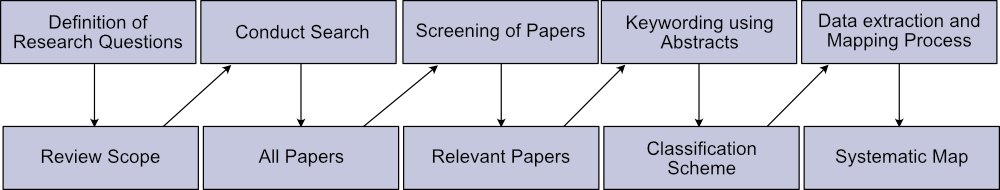
\includegraphics[width=\linewidth]{images/petersen_model.png}
  \caption{Process model (\cite{petersen2008})}
  \label{fig:mapping}
\end{figure}

% definition of research questions, 
The process begins by defining focused research questions that are aligned with
the goal of the study. The goal of the study often is to create a general
overview of the research area, and to identify the type and quantity of research
(\cite{petersen2008}). Unlike in more focused systematic literature reviews, the
research questions of mapping studies are less focused and cover a broader scope
(\cite{kitchenham2010}). For example, possible research questions on studies
could be: \emph{"Which are the most investigated quality aspects of the software
  requirements specifications techniques?"} (\cite{condori2009}) or \emph{"What
  efforts have been reported in literature for Software Engineering curriculum
  design, implementation, assessment and management?"} (\cite{qadir2011}). These
topic-oriented questions are often combined with research questions regarding
the meta-level information, such as publication year, venue, and research
methods (\cite{petersen2015}).

% conducting search, 
The next phase of the mapping is the initial material search, which can be
conducted multiple ways. Search strings can be formulated from the research
questions, and used on academic databases and search engines
(\cite{petersen2008}). For example, databases such as IEEE Explore and ACM, as
well as aggregators like Google Scholar can be utilized. As the search phrases
should be research question driven, following a criteria such as PICO might
prove to be helpful, as suggested by Kitchenham and Charters
(\cite*{kitchenham2007}). PICO (Population, Intervention, Comparison, Outcomes)
provides an frame to consider research questions' elements and identify
keywords. As the goal is to achieve broad overview of the research, study
outcomes are not taken into account, as this could result in a biased results
(\cite{petersen2008}). The search can also be conducted manually on specific
journals and conference proceedings that cover the target area
(\cite{petersen2008}). This approach is used in this thesis, as it enables
targeting specific reputable and well-known publication venues.

% screening of papers, 
After the initial material has been gathered, it is further refined by excluding
papers not relevant to answering the research questions (\cite{petersen2008}).
Separate criteria for both inclusion and exclusion is used to find the papers
fit for further analysis. According to Petersen, Vakkalanka and Kuzniarz
(\cite*{petersen2015}), the criteria may refer to relevance to the topic,
publication venue, time period, language restrictions, and evaluation
requirements. Considering evaluation requirements should be avoided with
systematic maps as it might limit recent trends. Once the criteria is decided,
it is applied to the titles and abstracts of the articles (\cite{petersen2015}).
In case of unclear or poor quality abstracts also the introduction and
conclusion sections of the article may be studied (\cite{petersen2008}). As no
full-text reading is required, screening of papers can be performed rapidly.

% keywording, 
Once the final set of papers is narrowed down and determined, keywording is
performed. As described by Peterson (\cite*{petersen2008}), The keywording
process starts by first by analyzing the research papers' abstracts by searching
possible frequent keywords and prevalent concepts from them. The keywords of
each paper are then combined together to achieve a more general set of concepts.
On some cases having a more detailed inspection of the article might be required
(\cite{petersen2008,petersen2015}). After the final set of keywords is chosen,
they are clustered into categories representing the article population
(\cite{petersen2008}). This emergent classification schema can then be used in
the data extraction phase.

Different research facets can be used in the classification. For example in
addition to the topical scheme emerging from the keywords, a topic-independent
facet reflecting the research approach can be used. One example of the latter is
the classification of research approaches by Wieringa et. al
(\cite*{wieringa2006}). Wieringa's classification categorizes scientific papers
into six categories such as validation research, solution proposals, and opinion
papers. Using existing topic-independent categorization also enables the
comparison of  different research fields (\cite{petersen2015}).

% data extraction and mapping.
In the final phase of the mapping process, the data extraction is performed by
sorting the papers into the classification schemes present
(\cite{petersen2008}). The schema may evolve during the data extraction process,
changing the categories to match the article population more accurately
(\cite{petersen2015}). The categorization based on the chosen facets results in
a frequency table, i.e. the mapping, with can then be presented with via
visualization and summary statistics. Visualization using for example bubble
plots is preferred, as it is a powerful way to represent the information and map
of the field (\cite{petersen2008}).


\section{Differences with systematic literature reviews}

Because the systematic literature mapping as a study methods is less known in
the field of software engineering, the typical differences between it and more
common secondary study method, systematic literature review, is presented here.
There is many common factors in both of the methods, and as Kitchenham et al.
(\cite{kitchenham2010}) state, \textit{"the distinction between mapping studies
  and conventional SLRs can be somewhat fuzzy"}. They also present a view that
mapping studies are just a different type of systematic literature review.

Similar to other secondary study methods, mapping study aims to summarize and
present the research performed in the past. Whereas systematic review focuses on
very narrow research questions, mapping study usually has multiple broader
questions(\cite{kitchenham2010}). Difference in scope breadth can also be seen
in the search strings, as the initial material search for mapping is likely to
return large number of studies (\cite{kitchenham2007, petersen2008}). Mappings
are usually conducted to achieve an overview of the research area, and therefore
the depth of the studies is not as great as in the SLRs. The mapping focuses
more on the thematic analysis of the articles instead of in-depth analysis of
their results or gathering empirical evidence based on their results, which is
often the goal of an traditional SLR (\cite{petersen2008}). Therefore the
quality of the objects of study is not relevant, unless the quality itself is
the aspect to be investigated.

Since both methods have their strengths and weaknesses, using them
complementarily can be an effective combination. As suggested by Petersen et. al
(\cite*{petersen2008}) and Kitchenham et al. (\cite{kitchenham2010}), good
approach is to first get an overview of the research area with systematic map,
and then applying conventional literature review to a specific focus area.
Results of the mapping can provide information on the quantity of available
evidence, which can help targeting the follow-up SLRs more precisely.


\section{Method choice}

As a thesis topic, Artificial General Intelligence is a challenging and broad
area. By focusing on the AGI research articles as an object of study, useful
research can still be performed without requiring too much prior knowledge and
expertise on the topic from the author. The reason behind the choice of
systematic literature mapping is that it fits specifically well on creating
overview of the study area. As the research questions of this thesis are broad,
mapping study is a more suitable approach than a conventional SLR.

Due to the complexity of the topic, it can be difficult to enter as a newcomer.
Kitchenham et al. (\cite*{kitchenham2010}) suggest that a systematic mapping of
the field can be useful to researchers new to the area.  It can also be useful
in introducing it to people unfamiliar with the field, both in academia and on
the industry's side. As can be seen from the history of AI research in
\ref{history}, AGI is also a topic that is known of it's fluctuating interest
and popularity, therefore seeing the temporal trends and state of the current
research can be of interest. Mapping study is a good way to achieve that.

The mapping process guidelines by Petersen et al.
(\cite*{petersen2008,petersen2015}) were chosen to be followed as they were the
most used ones in software engineering community (\cite{petersen2015}). Also the
most popular guideline for systematic literature review by Kitchenham et al.
(\cite*{kitchenham2007}) can be utilized to some degree because of the similarity
of the methods. These guidelines provide clear methodologies for the study. In
addition, the process can further utilize for example the scientific paper
classification scheme presented by Wieringa et al. (\cite{wieringa2006}), as it
provides an useful and straightforward research facet to the categorization
phase of the process.

To minimize the possible validity threats in this thesis and to try to prove its
rigor, the research method and it's execution is described in detail in chapters
\ref{chap:method} and \ref{chap:conducting}. However, as the study was was
conducted by one Master's student with limited time, the complete negation of
researcher bias especially in the material search and article exclusion phases
is not possible. As pointed out by Wohlin et al. (\cite*{wohlin2013}), the
reliability of secondary studies such as this mapping should not be taken for
granted.


\chapter{Conducting the literature mapping}
\label{chap:conducting}

In this chapter the systematic literature mapping is conducted following the
process described in section \ref{method_description}. To ensure that the study is
conducted with rigor, documenting it in detail is essential. This chapter only
describes the process, the actual results of the mapping are presented in
chapter \ref{chap:results}. Following the guidelines mentioned in section
\ref{method_description}, the following sections focus on each of the phases of
the study.

A search for similar literature studies was performed on University of
Jyväskylä's thesis archive JYX, Google Scholar, and Scopus, and no results were
found. Studies that were found were mostly conventional SLRs with much more
narrow scope. It was concluded that there exists no similar mapping study on the
topic.

\section{Research questions}

The following research questions aim to cover the goal of the study, to create
an overview of the scientific research performed on the field of AGI.

\begin{itemize}
  \item[RQ1:] How much, and what kind of research is done in the field of AGI?
  \item[RQ2:] Where and when were the studies published?
  \item[RQ3:] What are the major research topics in the field and have they
        changed over time?
\end{itemize}

The first question focuses on the type and volume of the published AGI related
research. The second question focuses on the publication venue and time of the
articles, showing temporal trends and popular forums for the topic. Research
question three aims to find out the most popular subtopics and their change in
the study's time frame. The answers to these questions will be presented in
chapter \ref*{chap:results}.


\section{Material search}

This thesis utilized both manual and broad automatic search in the material
gathering. The targeted publication venues are either very topic specific, or
otherwise high-ranked in the artificial intelligence community, and general
content-wise. The following venues are used in this thesis:

\begin{itemize}
  \item \textbf{Journal of Artificial general intelligence} (journal)
  \item \textbf{Artificial Intelligence} (journal)
  \item \textbf{Journal of Artificial Intelligence Research} (journal)
  \item \textbf{International Conference on Artificial General Intelligence}
        (conference)
  \item \textbf{International Joint Conference on Artificial Intelligence}
        (conference)
\end{itemize}

%TODO: publication forum guidelines should be looked through
One basis for the selection of publications was the Finnish Publication Forum
(\cite{jufo}) ranking. In this thesis Publication Forum is referred as JUFO.
Publication Forum ranks peer-reviewed scientific publication venues on grades
1-3, with 1 being the standard level, and 3 being the highest.

The reasoning behind venue choices were as follows: Journal of Artificial
general intelligence (JAGI) (JUFO rank 1) and International Conference on
Artificial General Intelligence (ICAGI) are very topic specific, and therefore
should contain the most relevant information within the field. These main forums
are likely to contain most of the research articles. Artificial Intelligence
journal (AIJ) and Journal of Artificial Intelligence Research (JAIR) were chosen
because they have the highest JUFO ranking and therefore are leading
publications of the AI field. Both also have high citescore (7.7 and 6.4
respectively) considering they do not focus on any specific subfield of AI. For
the same reason, International Joint Conference on Artificial Intelligence
(IJCAI) was included (JUFO rank 2). These more general sources may not contain
many papers as the topic-specific publications, but can show the relative
popularity of the field within the AI research.

% Why journals were chosen, information about them, reliability, area coverage,
% jufo rankings etc. Reasoning behind choosing specific journals instead of just
% all-covering database searches? More text about publication forum and
% publication relability

Out of these, Journal of Artificial General
Intelligence (JAGI) was searched manually due to low quantity of articles, but
otherwise automatic search was performed using search engines Scopus and
Springer Link.

The search phrases for the automatic search were derived from the research
questions, following the aim of this study. Included were the close concepts
similar to AGI, such as HLAI and superintelligence. The logical search phrase
used was " \emph{"artificial general intelligence" OR agi OR "human-level ai" OR
HLAI OR superintelligence} ". The phrase is very broad and non-restricting, but
this helps it yield results even in more general venues.

The publication interval of the papers was limited to years \textbf{2015-2019}
to reduce the material to reasonable quantity. This choice prevents seeing
temporal trends that might not show in such a short interval, but longer time
frame was not viable considering this is only a master's thesis.

\section{Choosing papers for inclusion}

The initial material search was performed during October 2020. The papers found
on the search were further narrowed down using the following criteria. All
literature accepted for this thesis needed to be:

\begin{itemize}
  \item presenting and/or relating to Artificial General Intelligence,
        Human-level AI, or similar concept of general intelligence,
  \item written in English,
  \item published between 2015-2019,
  \item a peer-reviewed journal or conference paper, and
  \item available digitally free or as a member of University of Jyväskylä.
\end{itemize}

Piece of literature would be excluded if it was:

\begin{itemize}
  \item a book, a thesis, or lecture notes,
  \item not wholly available digitally or
  \item a duplicate of already included paper.
\end{itemize}

For a paper to be found relevant to the topic, it needed to clearly reference
the concept of (artificial) general intelligence in its title or abstract, with
intention of relating the article to it. If the concept is only mentioned as a
sidenote or as an example without further relevance, it should be excluded. If a
clear decision couldn't be made from these parts, article could be further
examined. In case of duplicate articles or articles concerning the same study,
only the latest one is included in the study.

The initial search yielded total of 187 papers. Almost all of the initial
results fulfilled the meta-level criteria as the used search engines (Scopus and
Springer Link) offered extensive filtering capabilities. These results were then
inspected in two separate phases. In the first phase, the titles and abstracts
of the articles were examined, and then the article was marked as either
excluded or potential in a spreadsheet. After this initial inspection, 122
papers were considered potential, and would be subject of further inspection.

In the second phase, the potential papers were examined again, with the research
questions and inclusion criteria considered more thoroughly, to further exclude
papers that were not relevant to the topic. During this phase, a small example
set of excluded and included papers was sent to the thesis supervisor to confirm
their categorization. During this phase it became apparent that without stricter
inclusion criteria the amount of accepted papers would be excessively high. It
was decided that to be included, the article would have to explicitly relate
itself to general intelligence. In the end, 92 papers were included and would be
used as the mapping sample. Table \ref*{table:forumtable} shows the number of
accepted papers and their publication venues.

  \begin{table}[H]
    \footnotesize
    \centering
    \begin{tabular}{|l|l|l|l|l|}
      \hline
      \textbf{Publication forum}  & \textbf{Total results} & \textbf{Potential results} & \textbf{Accepted results} & \textbf{Accepted results (\%)} \\ \hline
      JAIR   & 5   & 3  & 2  & 40\%  \\ \hline
      IJCAI  & 12  & 8  & 4  & 33.33\%  \\ \hline
      AIJ    & 3   & 3  & 1   & 33.33\%  \\ \hline
      JAGI   & 15  & 9  & 6   & 40\%  \\ \hline
      ICAGI  & 152 & 99 & 79  & 51.97\%  \\ \hline
      \textbf{All} & \textbf{187} & \textbf{122}  & \textbf{92}  & \textbf{49.20\%}  \\ \hline
    \end{tabular}
    \caption{Publication forums and their results}
    \label{table:forumtable}
  \end{table}

\section{Keywording}
Once the articles were narrowed down to to those relevant to topic, they were
inspected more thoroughly and the emergent concepts or keywords were extracted.
These keywords were then further combined to topic categories until no further
merging could be done without making them too general and losing too much
information in the process. The resulting categorical scheme of 22 distinct
topic categories is illustrated in Table \ref{table:topicdescription} in the
results chapter.  

\section{Data extraction and mapping}

In the actual data extraction phase, the included research articles were sorted
into two different categorization schemes. First one was the topic
categorization that emerged from the papers themselves, and the other one was
the topic-independent categorization presented by Wieringa et al.
(\cite*{wieringa2006}). The latter enables us to make comparisons with AGI and
other fields of research that aren't necessarily related. It also provides
information on the kind of research done, answering RQ1. Wieringa's scheme is
presented in Table \ref{table:wieringa}.

\begin{table}[H]
  \footnotesize
  \centering
  \begin{tabular}{p{0.30\linewidth} p{0.70\linewidth}}

    \textbf{Class}  & \textbf{Class description}  \\ \hline
    Evaluation research & Investigates existing problem or technique in practice with sound research methods. \\ \hline
    Validation research & Investigates a solution proposal not yet implemented in practice using sound research methods. Prototypes, simulations or mathematical proof are among possible methods. \\ \hline
    Solution proposal & Paper proposes a new solution to a problem, with arguments for its relevance. Solutions must be novel or significantly improve existing ones. \\ \hline
    Philosophical papers & Conceptual frameworks and new viewpoints on the topic. \\ \hline
    Opinion papers & Papers presenting author's personal opinion on the topic. \\ \hline
    Personal experience papers & Present author's experience on something that has been done in practice. Doesn't necessarily provide evidence. \\ \hline

  \end{tabular}
  \caption{Article classification by Wieringa et al. (\cite*{wieringa2006})}
  \label{table:wieringa}
\end{table}

The papers could belong to multiple categories on both schemes. This enables
inspection of connections between the topics that are often met together. The
results of this mapping process are presented in the following chapter.

The initial inspection of articles was performed online. Once the paper
inclusion process was complete, the final set of articles was downloaded for
further local inspection. The data about the articles was kept in a spreadsheet
document. Graphs in this thesis were plotted with either \LaTeX or with Python
scripts, using libraries such as Matplotlib and Plotly.

%============== RESULTS ===============

\chapter{Results and analysis}
\label{chap:results}

 In this chapter the results of the literature mapping are presented. Answers to
 research questions are discussed, and observations made during the study are
 shown. 

 \section{Publications years and venues}

 As the field of Artificial General Intelligence is relatively small when
 compared to other branches of AI research, it is very focused on specific
 publication forums. This can be seen evidently from the sample papers'
 publication venues. Figure \ref*{fig:forumpie} shows that almost 86\% of the 92
 sample articles were published as the proceedings of the Internation Conference
 on Artificial General Intelligence. The second largest concentration of
 articles was on the Journal of Artificial General Intelligence, as was expected
 it being the only non-conference publication on the topic. It needs to be also
 noted that even though Artificial Intelligence Journal and Journal of
 Artificial Intelligence Research are esteemed journals that contribute hundreds
 of AI articles every year, their articles only constituted less than four
 percent of this study's papers. 


 \begin{figure}[H]
  \centering
  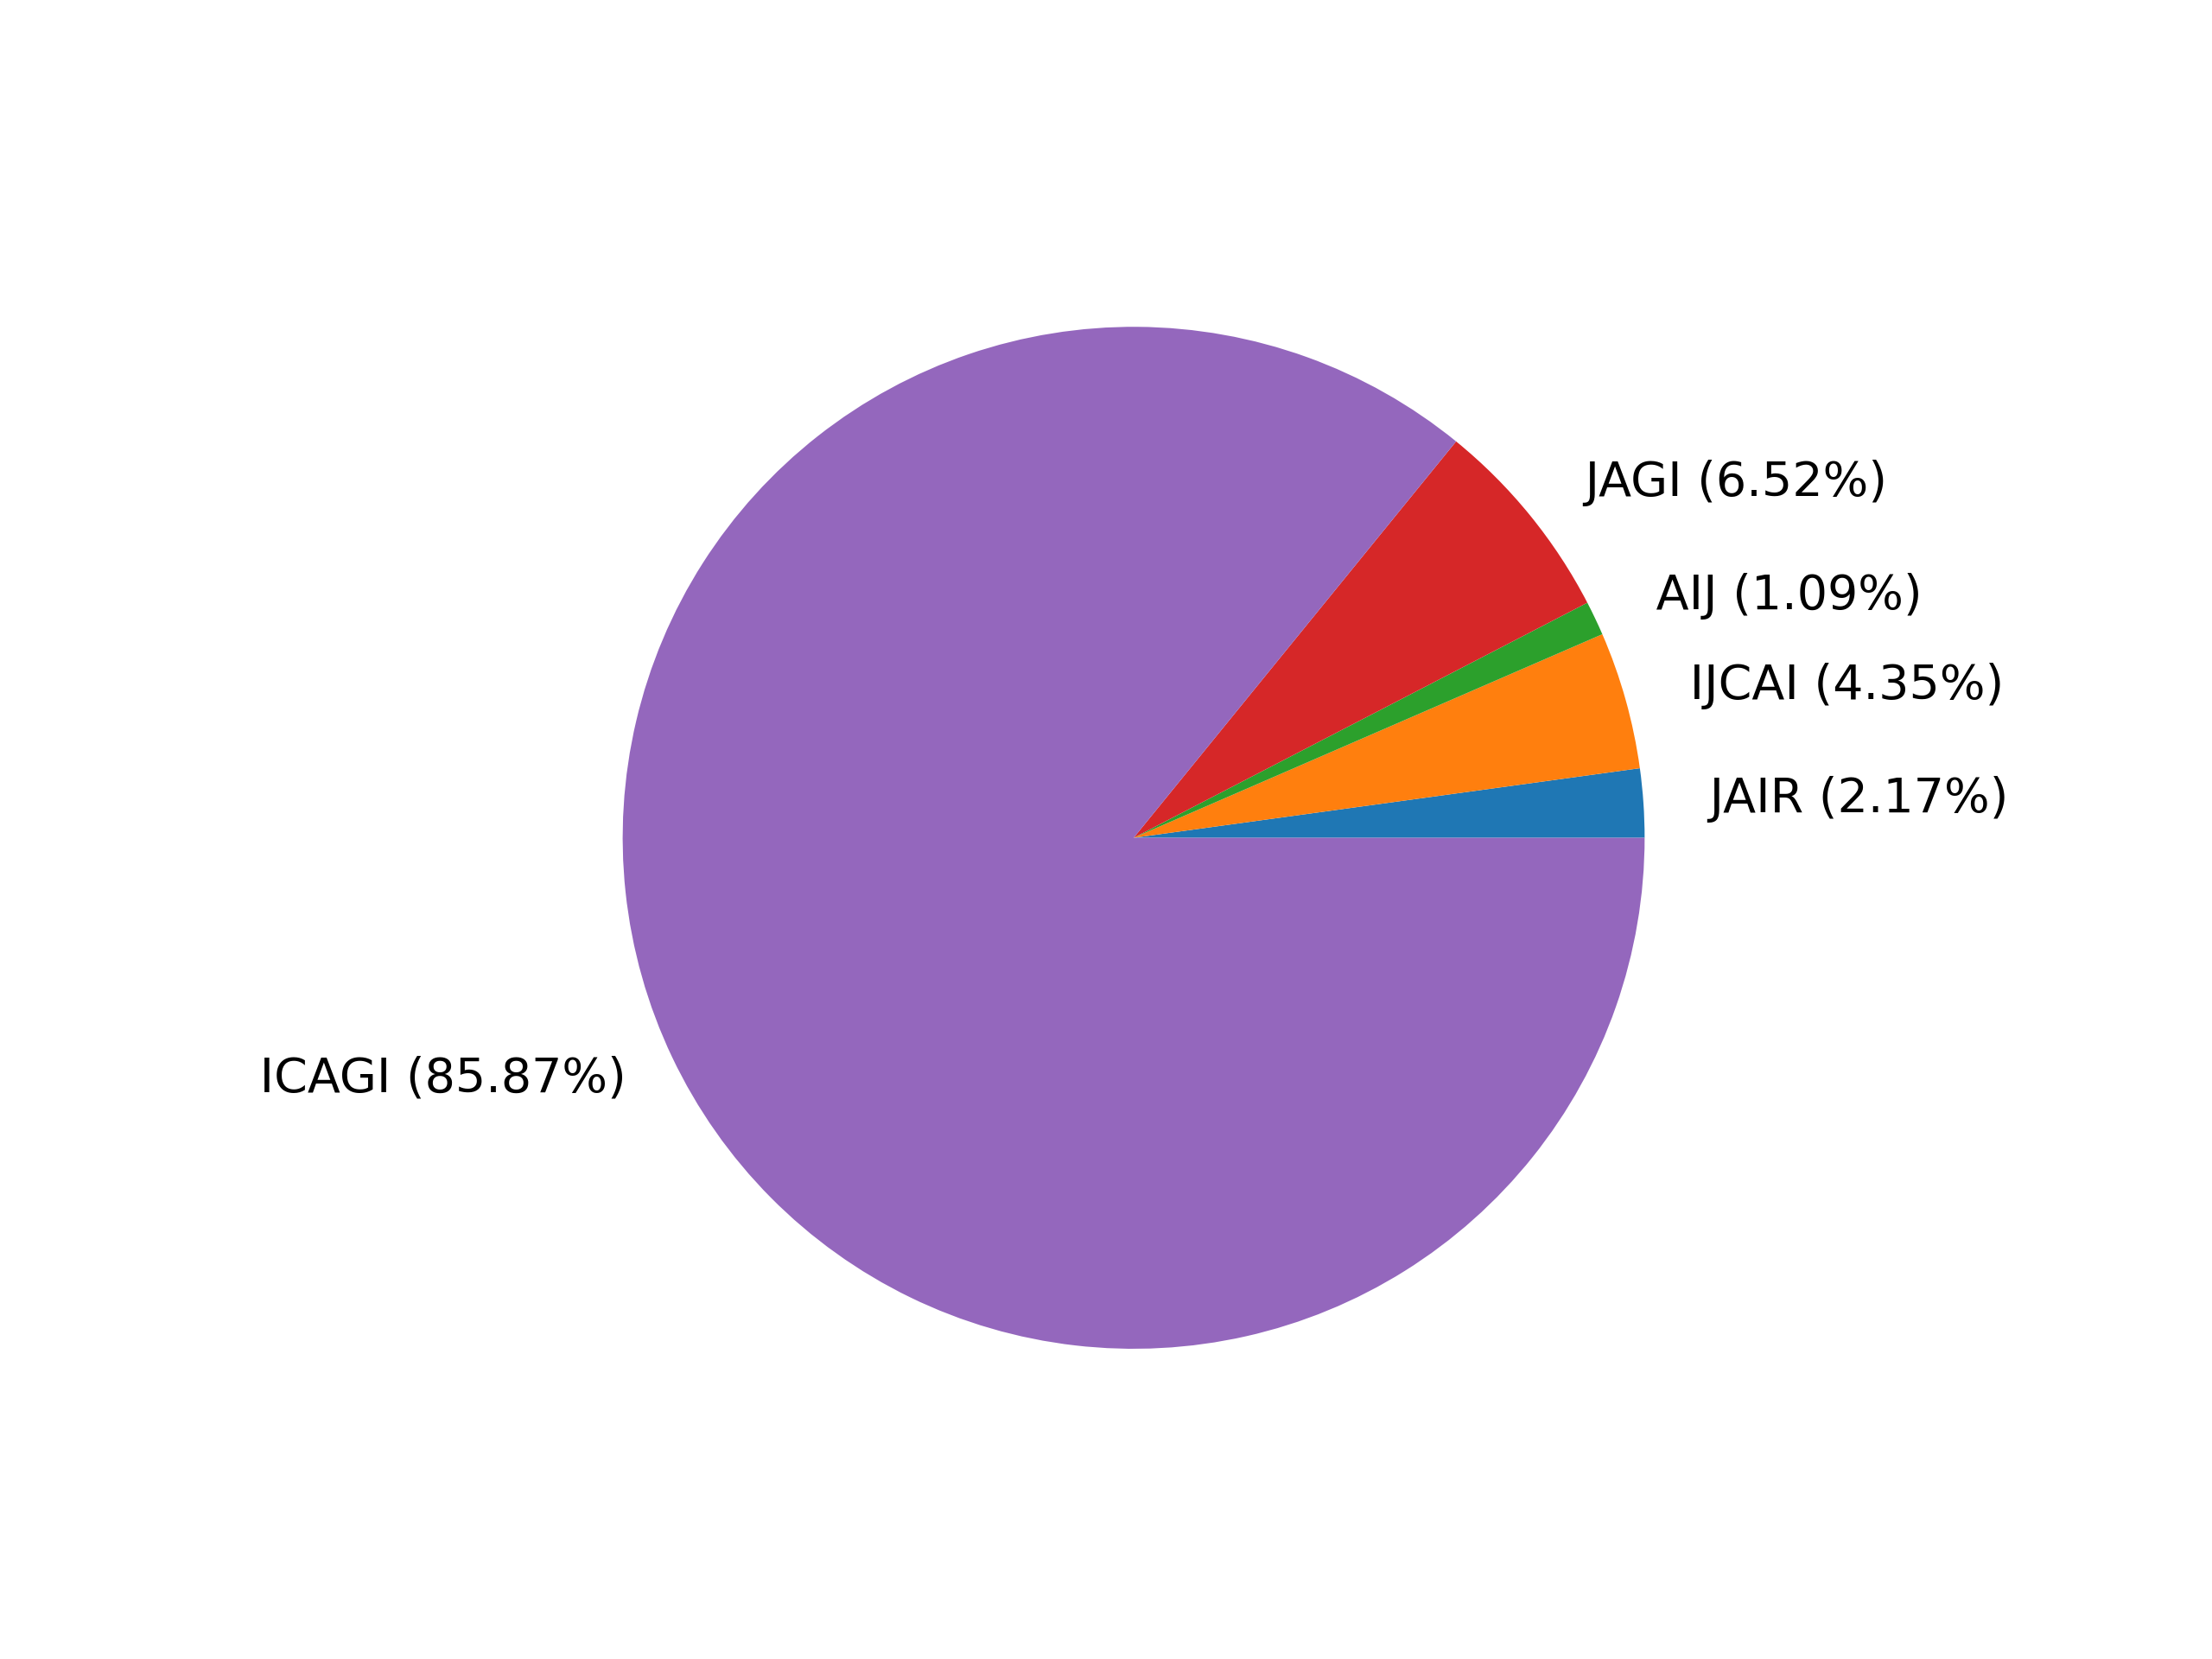
\includegraphics[scale=0.70]{material/data/forum_pie.png}
  \caption{Article distribution between the publication forums}
  \label{fig:forumpie}
\end{figure}

In Figure \ref{fig:yearlybar} the amount of yearly published articles and their
venues are visualized in a bar plot. As the inspected time period on this thesis
is short, only five years, predicting temporal trends accurately is not
possible. However, it can be seen that every year there is steady publication
pace of at least 13 articles, with the average being 18.4 a year. In year 2018
25 different articles were published, which was the highest number during the
inspection period.

ICAGI is the \emph{"only major conference series devoted wholly and specifically to
the creation of AI systems possessing general intelligence at the human level
and ultimately beyond"} (\cite{icagihome}). It has been organized yearly since
2008.

Therefore to answer research question RQ2, it can be said that while there are
AGI studies being published in different publication forums, vast majority of
the research is released as yearly conference proceedings of International
Conference on Artificial General Intelligence. Research community is active but
small, as only average of 18,4 articles fitting this scope are published yearly.

\begin{figure}[H]
  \centering
  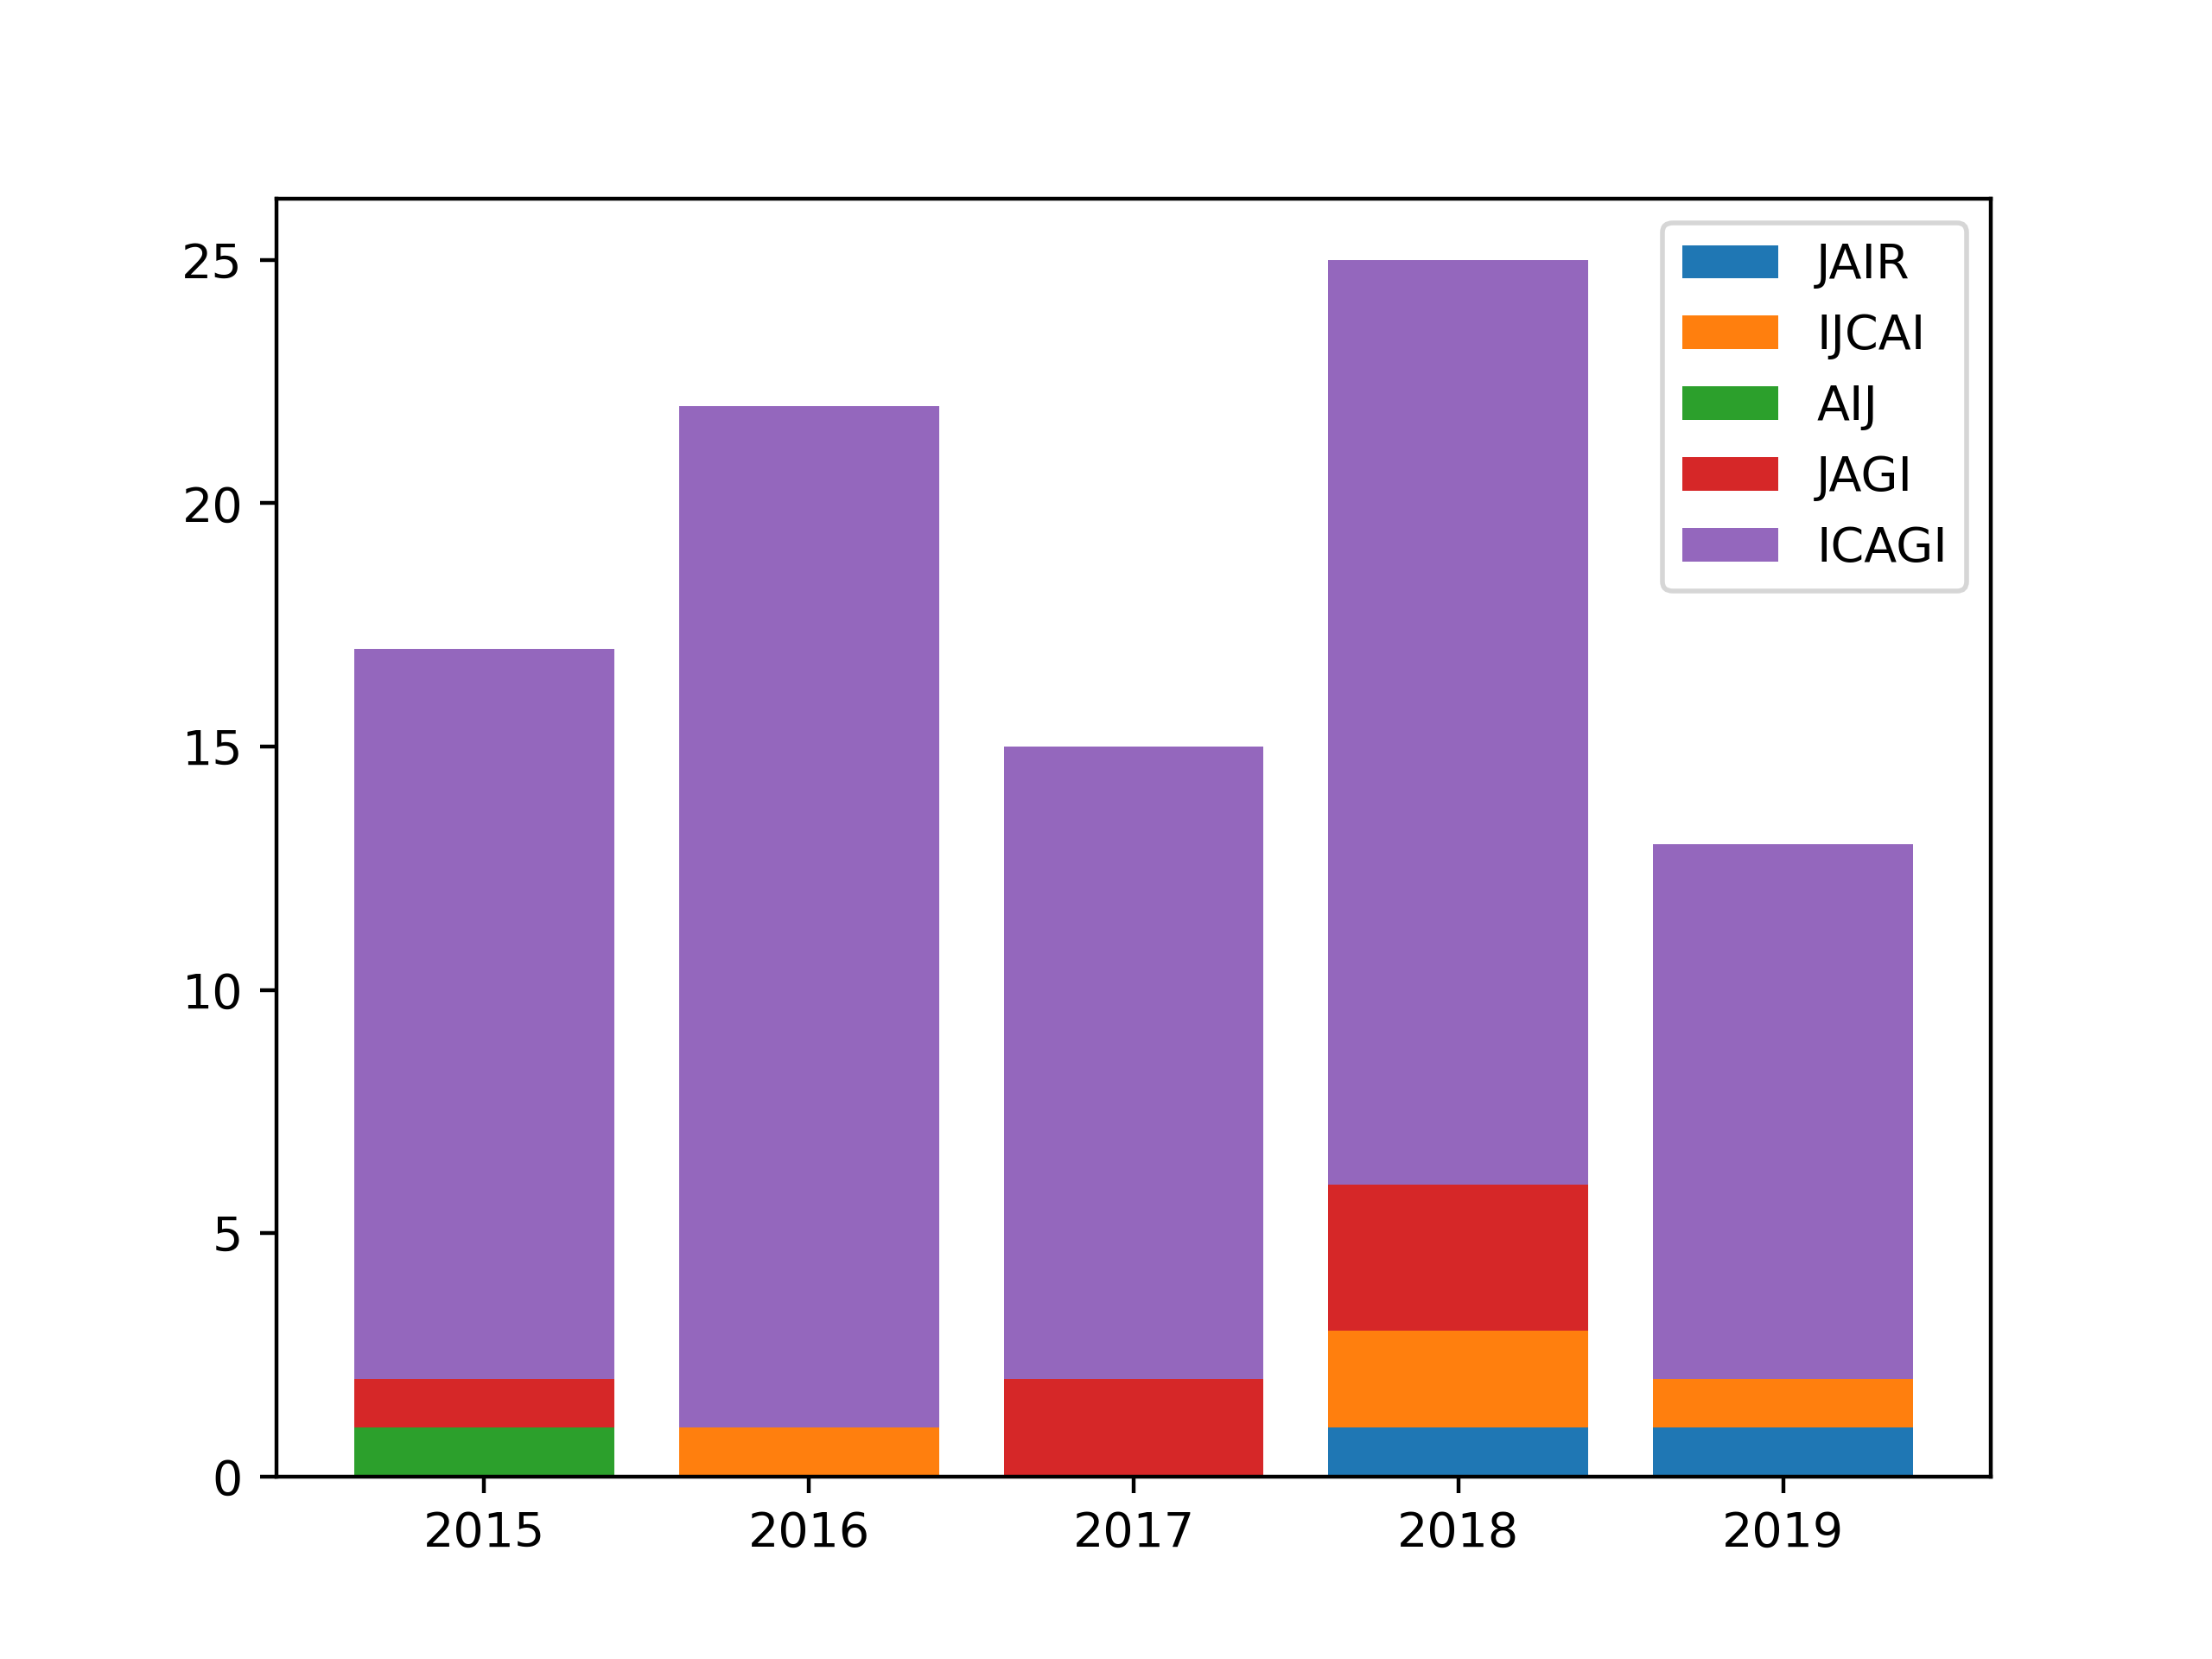
\includegraphics[scale=0.60]{material/data/yearly_publications.png}
  \caption{Yearly articles by publication forum}
  \label{fig:yearlybar}
\end{figure}

\section{Common research topics}

The main goal of this thesis was to achieve an overview of the AGI field.
Through the mapping process, 22 different topic categories were found, and they
are presented in Table \ref{table:topicdescription}. A single paper can relate
to multiple topics. These topics show us how the AGI research is focused on the
top level. From the amount of different topics it can be seen that the research
area is broad and not focused on a single style of solutions. 

From the sample articles, four different themes could be identified. These
themes are just high-level observations by the author based on the found topic
categories. \textbf{Building AGI systems} is of course naturally a very
prominent one. These papers were more focused on the possible theory and
implementations that could be used in building of an AGI system: how it reasons
and plans, how capabilities like perception could be implemented, and how to
handle issues like combinatorial explosion. One reoccurring theme was
\textbf{Learning}. Different approaches to more common machine learning
techniques like reinforcement learning and algorithms related to it like
Q-learning and Deep Q-Networks are demonstrated. In additions to this, research
on cumulative learning, lifelong learning, and episodic memory is very
prominent. Third theme was \textbf{Agent interaction}, meaning topics such as
multi-agent systems, environmental interaction, and human-computer interaction.
Lastly there are \textbf{Non-technical topics}, such as philosophical
questions, AI ethics, emotion in AI and meta-level research.

\begin{table}[H]
  \footnotesize
  \centering
  \begin{tabular}{p{0.05\linewidth} p{0.30\linewidth} p{0.65\linewidth}}

    \textbf{\#} & \textbf{Category}  & \textbf{Category description}  \\ \hline
    1  & Cognitive architectures & Cognitive architectures and their descriptions.  \\ \hline
    2  & AGI Design & General ideas on how AGI or its components could be designed and implemented. \\ \hline
    3	 & Reasoning and Inference &  Approaches on temporal and causal reasoning and inference techniques. \\ \hline
    4	 & Planning and decision making & Utilizing existing knowledge in planning and decisions. \\ \hline
    5	 & Probabilistic approaches & Probabilistic approaches e.g. Bayesian techniques and uncertainty handling.\\ \hline
    6	 & Category theory & Approaches relating to category theory.\\ \hline
    7	 & Universal AI & Concepts relating to Universal AI (\cite{hutter2004}): universal induction, AIXI, compression.\\ \hline
    8	 & Physical robots & Physical robots and interaction with physical environment. \\ \hline
    9	 & Computer vision and perception & Topics concerning vision and perception systems of an agent.\\ \hline
    10 & Nature-inspired approaches & Artificial animals, homeostatic agents and other nature-inspired ideas.\\ \hline
    11 & Reinforcement learning & Topics directly relating to reinforcement learning, e.g. Q-learning, rewarding techniques.\\ \hline
    12 & Recursive self-Improvement & Relating to fast self-improvement of an agent and intelligence explosion. \\ \hline
    13 & Experiential learning & Cumulative learning, artificial pedagogy and other topics related to how agent builds on existing knowledge.\\ \hline
    14 & Agent environment & Descriptions of environments and how agents interact within them.\\ \hline
    15 & Multi-agent systems & Topics relating to agent-to-agent interaction and cooperation.\\ \hline
    16 & Human-computer interaction & How human and agent interact and communicate and their relation to each other.\\ \hline
    17 & AI safety & Approaches on how to safely create and interact with AGI, and what safety issues arise alongside general intelligence.\\ \hline
    18 & Philosophical aspects & Philosophical questions relating to artificial intelligence, e.g. AI ethics and morality.\\ \hline
    19 & Human-like qualities & Approaches with basis on human qualities like emotion and empathy.\\ \hline
    20 & AGI research & Secondary research about AGI research. \\ \hline
    21 & AI evaluation & How to evaluate and measure AI intelligence and performance.\\ \hline
    22 & Game playing  & Game playing as a tool in development and evaluation of general agents.\\ \hline

  \end{tabular}
  \caption{Emergent topic categories}
  \label{table:topicdescription}
\end{table}

% Most researched ones explained. RQ3

In Figure \ref*{fig:topicbar}, the frequencies of research topics is presented
over the years. The most researched topic is \textbf{Cognitive architectures}.
Cognitive architecture means an abstract model of cognition as well as its
software implementation, which aims to be a system showing intelligent
behaviour, artificial intelligence (\cite{lieto2018}). In AGI research there are
few cognitive architectures that are standing out in the field. Goertzel's
OpenCog framework (See section \ref*{definition}) was seen in 8 different
papers, e.g Goertzel's idea of bridging the gap between theory and practice in
AGI design (\cite{goertzel2017agents}) and Potanov's attempt to create semantic
vision system by combining OpenCog with YOLOv2 object detection system
(\cite{potapov2018}). In addition to OpenCog, Non-Axiomatic Reasoning System
(NARS), developed by Pei Wang, was part of many articles. For example, besides
the introduction of its implementation (\cite{hammer2016opennars}), papers
describing its approach to emotion (\cite{wang2016emotional}) and inferential
learning (\cite{wang2016learning}). While many of these cognitive architecture
articles were mainly focused on presenting authors' system's implementation,
some were offering ideas that could be used in any other approaches to AGI.
These articles, among other papers focusing on not-implementation-specific
ideas, were categorized also to \textbf{AGI design} category that included 6
papers.

The second largest topic category was \textbf{Universal AI}. The theory of
universal AI was created by Marcus Hutter (\cite*{hutter2004}) and it describes
a complete mathematical model for general artificial intelligence, named AIXI
(\cite{hutter2012decade}). Although incomputable, this theory and topics related
to it are target of vigorous research. In this category there is 14 articles
concerning AIXI, Solomonoff's universal induction, functional programming and
compression. For example in 2019 paper by Franz, Gogulya and Löffler
(\cite*{franz2019william}), a monolithic inductive approach to AGI was
presented, taking advantage of AIXI and incremental compression techniques. In
(\cite{martin2016death}), death was formally defined to generally intelligent
agents like AIXI and discoveries were made regarding agents' behaviour in such
situations.

\textbf{Reinforcement learning} (RL) is the third largest category with 11
articles relating to it directly. As can be seen from the topic heatmap in
figure \ref{fig:topicheat}, it is technique associated with wide range of other
topics. In 2016 paper Susumu Katayama presents a new RL algorithm idea with
similarity to AIXI (\cite{katayama2016ideas}). It involves usage of
MAGICHASKELLER, research group's inductive programming system.

\textbf{Experiential learning} means that an agent utilizes it's previous
experiences in its actions, incrementally increasing its knowledge
(\cite{thorisson2019cumulative}). This type of learning enables agent to
generalize its abilities continuosly, making it one of the necessary
requirements of AGI. 11 articles with this topic were found, with some defining
new concepts such as cumulative learning (\cite{thorisson2019cumulative}), some
researching novel techniques like imitation learning (\cite{katz2016imitation}),
and some focusing on how to teach cumulatively learning agents systematically
via artificial pedagogy (\cite{bieger2017pentagon}).


Many papers with less technical topics such as \textbf{AI safety} and
\textbf{Philosophical aspects} could be found in the study, both prevalent in 11
papers. Especially focused topic was AI safety, which concerns problems like how
can we make sure AGI has the same desirable ethical values as its creators, how
can a superintelligent agent be contained safely, and how we can be sure that
the AGI accomplishes its goals without using possibly harmful unintended
shortcuts. These questions are generally referred respectively as \emph{the
alignment problem, the containment problem, and the problem of perverse
instantiation}. In (\cite{babcock2016containment}), necessary requirements are
identified for AGI containers to solve the containment problem. In 2019 paper,
Aliman and Kester present a novel ethical framework called \emph{Augmented
Utilitarianism} to alleviate the problem of perverse instantiation
(\cite{aliman2019augmented}). As can be seen from the quantity of papers
relating to AI safety, it is clear that this is one of the main issues that
needs to be solved in the creation of AGI.

The philosophical papers that weren't directly concerned with AI safety were
either discussing the ethics of AI or concepts like \emph{understanding} and
\emph{intelligence} itself. For example, in (\cite{thorisson2017understanding}),
the relationship between understanding and common sense is discussed, and in
(\cite[]{weinbaum2016Oopenended}), a new way of looking at the intelligence,
titled \emph{Open-Ended Intelligence}, is introduced as a novel approach to AGI.


\begin{figure}[H]
  \centering
  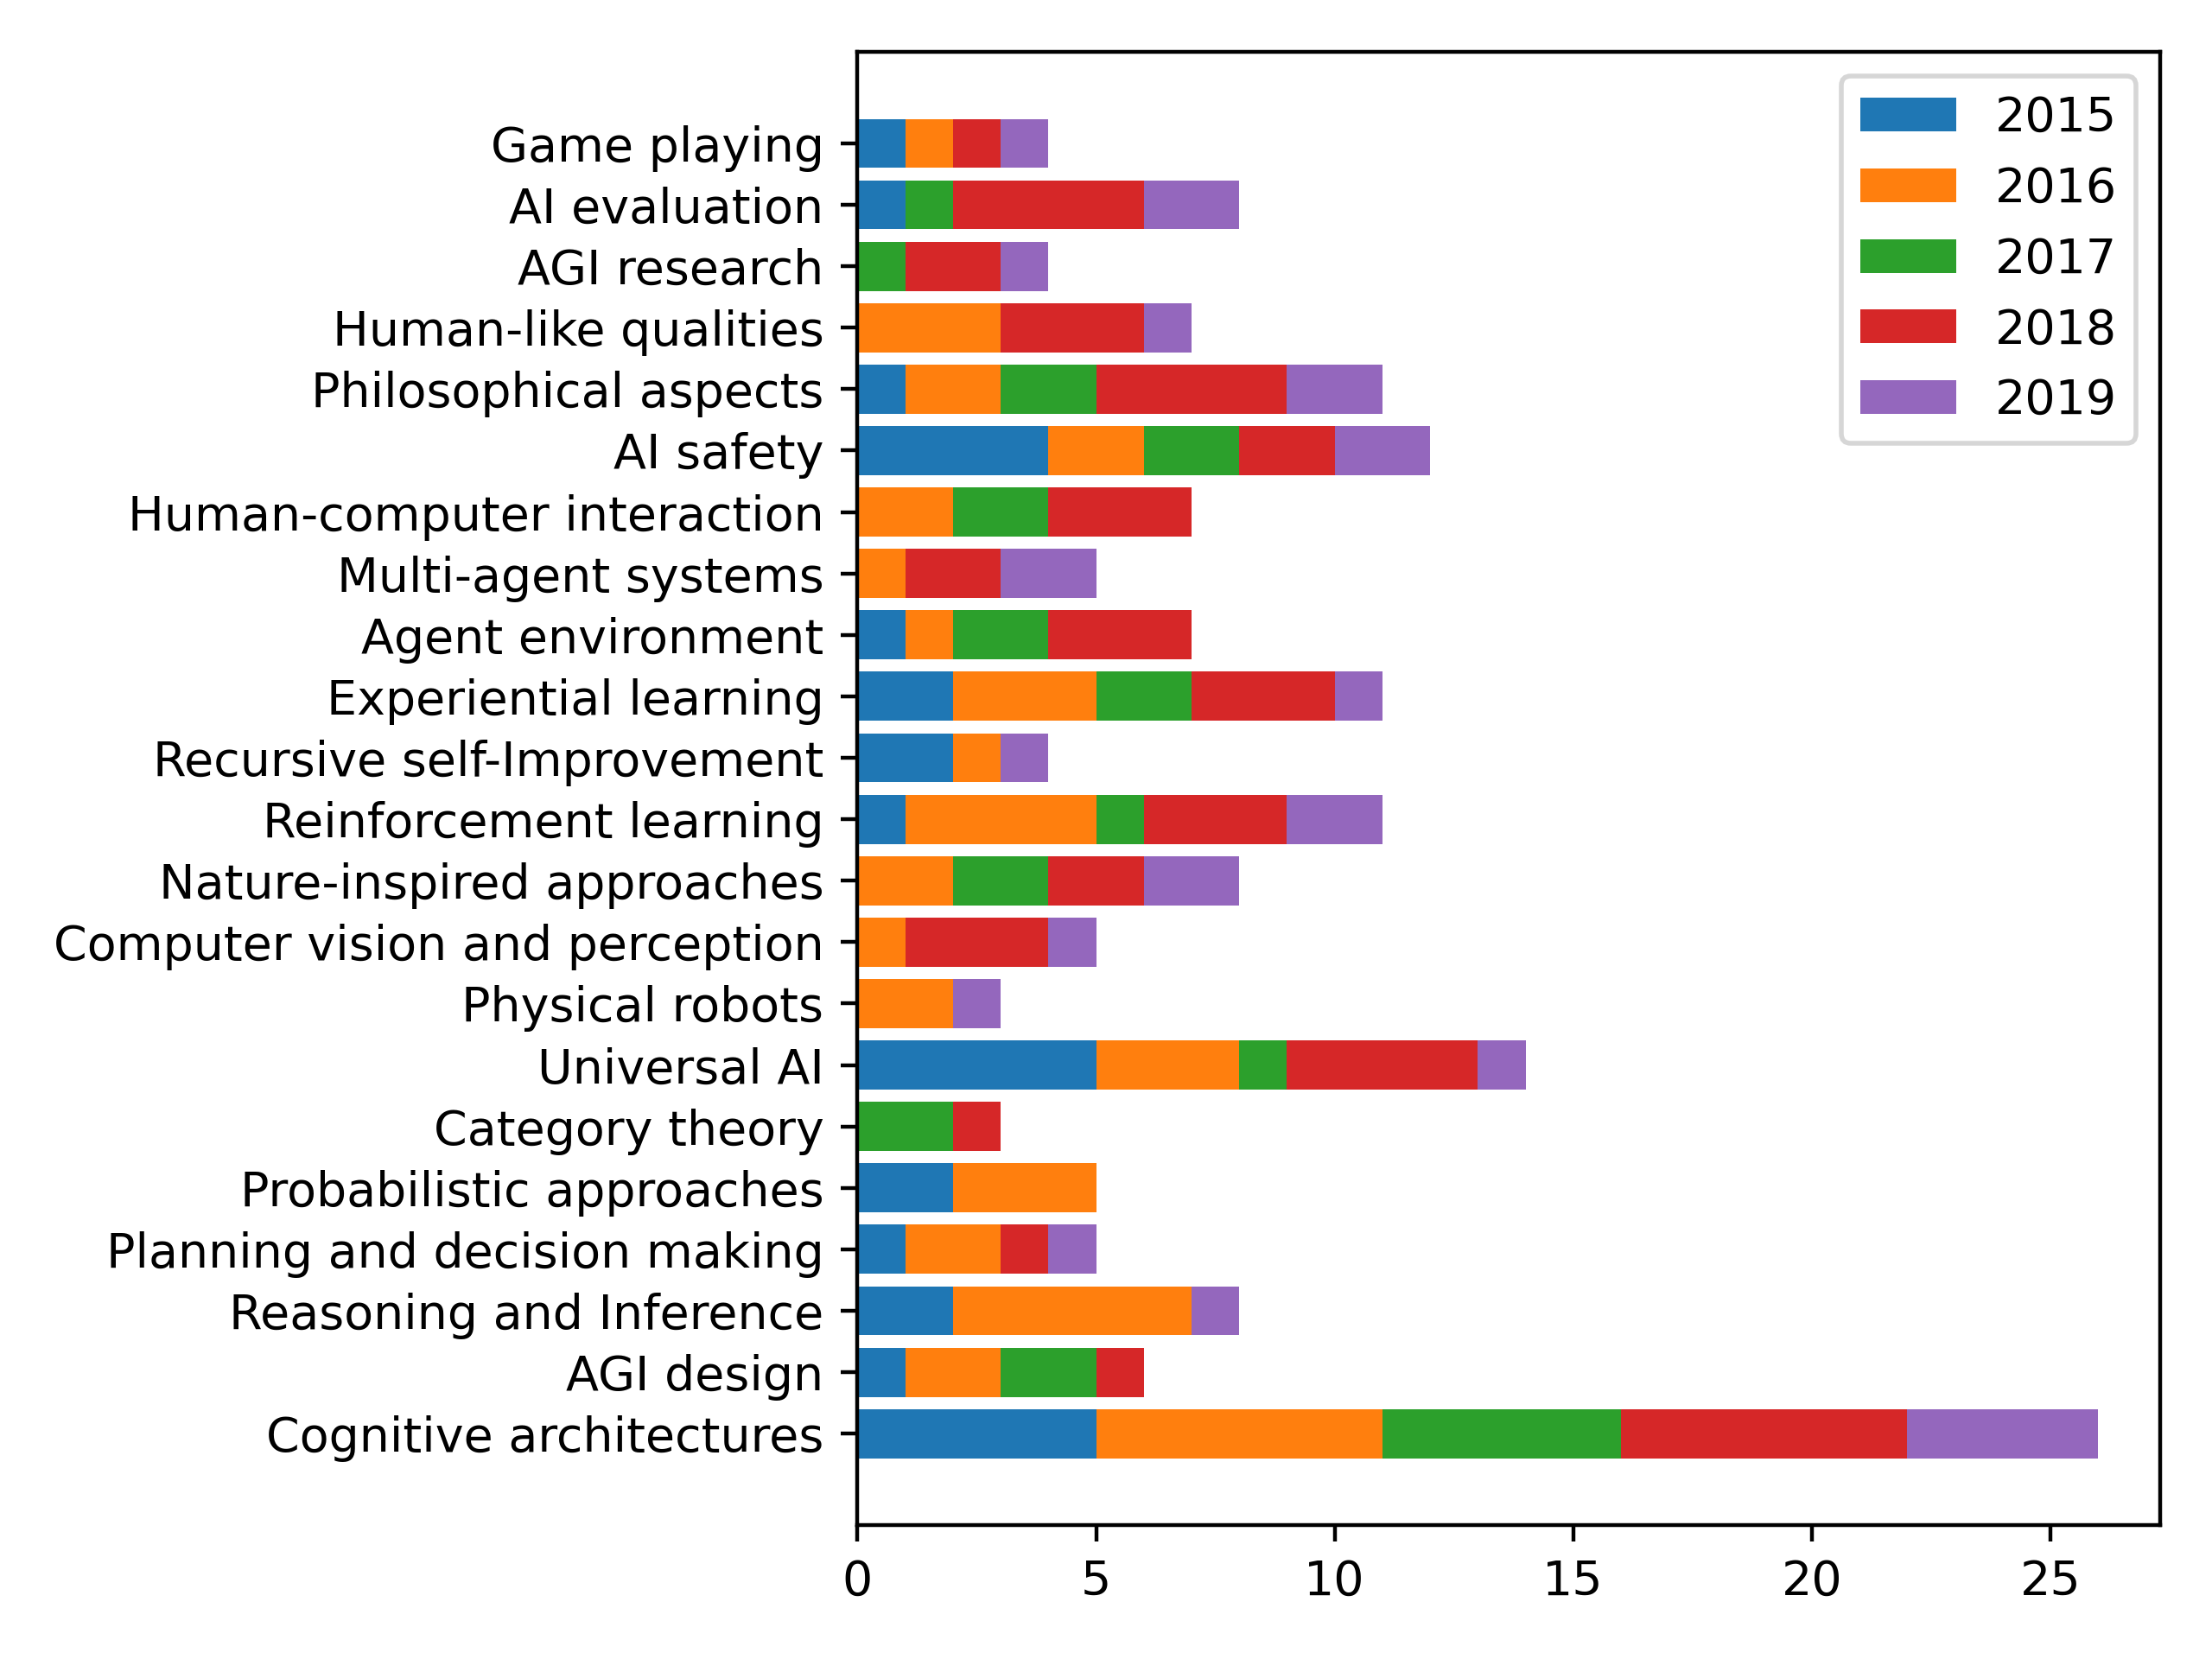
\includegraphics[scale=0.8]{material/data/topic_frequencies_by_year.png}
  \caption{Topic category frequencies}
  \label{fig:topicbar}
\end{figure}

% Short time trends
\section{Temporal trends}

Due to the limited time span, it is difficult to observe long term trends in AGI
research. However, some short time observations can be made from the yearly
publications in figure \ref{fig:topicbar}. 

Year 2019, the last one included in the study, had a major drop in published
articles in comparison with the previous year, from 25 to 13. In 2019, many
topics that were prominent on the previous years, e.g. universal AI, agent
environment, and human-computer interaction, dropped to only one or zero
articles published. Suprisingly there are some topics that don't have any
relating papers published in recent years, but each have one on 2019. This is
the case of recursive self-improvement, physical robots, and reasoning and
inference, each have only one paper published since 2016.

Few of the most common topics like AI safety, philosophical aspects, and
cognitive architectures have a regular publication pace, with approximately same
number of articles published every year, even in the slower years of 2017 and
2019. Other popular topics such as experiential learning and universal AI show
much more fluctuation in the yearly number of articles published.

Interestingly articles about probabilistic approaches have not been published
since 2016, which suggests that interest towards that particular approach is
decreasing.


% Relation to other topics
\section{Connections between topics}

Figure \ref{fig:topicheat} shows the relations between the topic categories. As
could be expected, cognitive architectures can be associated with as many as 15
other categories. As the aim of cognitive architecture is often to create a
versatile general agent, it is reflected on the way the research is done.
Interestingly nature-inspired approaches is often associated with agent
environment and reinforcement learning topics. One explaining factor is the
subject of artificial animals, animats, that were discussed in three articles.
Animats are homeostatic reinforcement learning agents that interact with their
environment. 

The relation between AI evaluation and universal AI can also be observed, with
three related articles. As universal AI deals with computability and similar
subjects, their mathematical evaluation might be more viable than other
approaches. Two of the three articles were authored by Ond\v rej
Vadinsk\'y (\cite*{vadinsky2018lessons,vadinsky2018sema}), and were focused on the
Algorithmic Intelligence Quotient test, designed for intelligent agent
evaluation.

One clearly visible focus area on the topic relations is the area with topics
15-20. The heatmap shows close connections between less technical topics such as
human-computer interaction, AI safety, philosophical aspects, and human-like
qualities, and also multi-agent systems and AGI research. This shows how
discussing AI safety requires also discussing how humans and computers interact,
and how abstract and difficult concepts like ethics, values and emotions can be
represented and conveyed to the machine. Two out of three secondary research
articles were targeting this focus area, so there is undeniably interest in
these topics.


\begin{figure}[H]
  \centering
  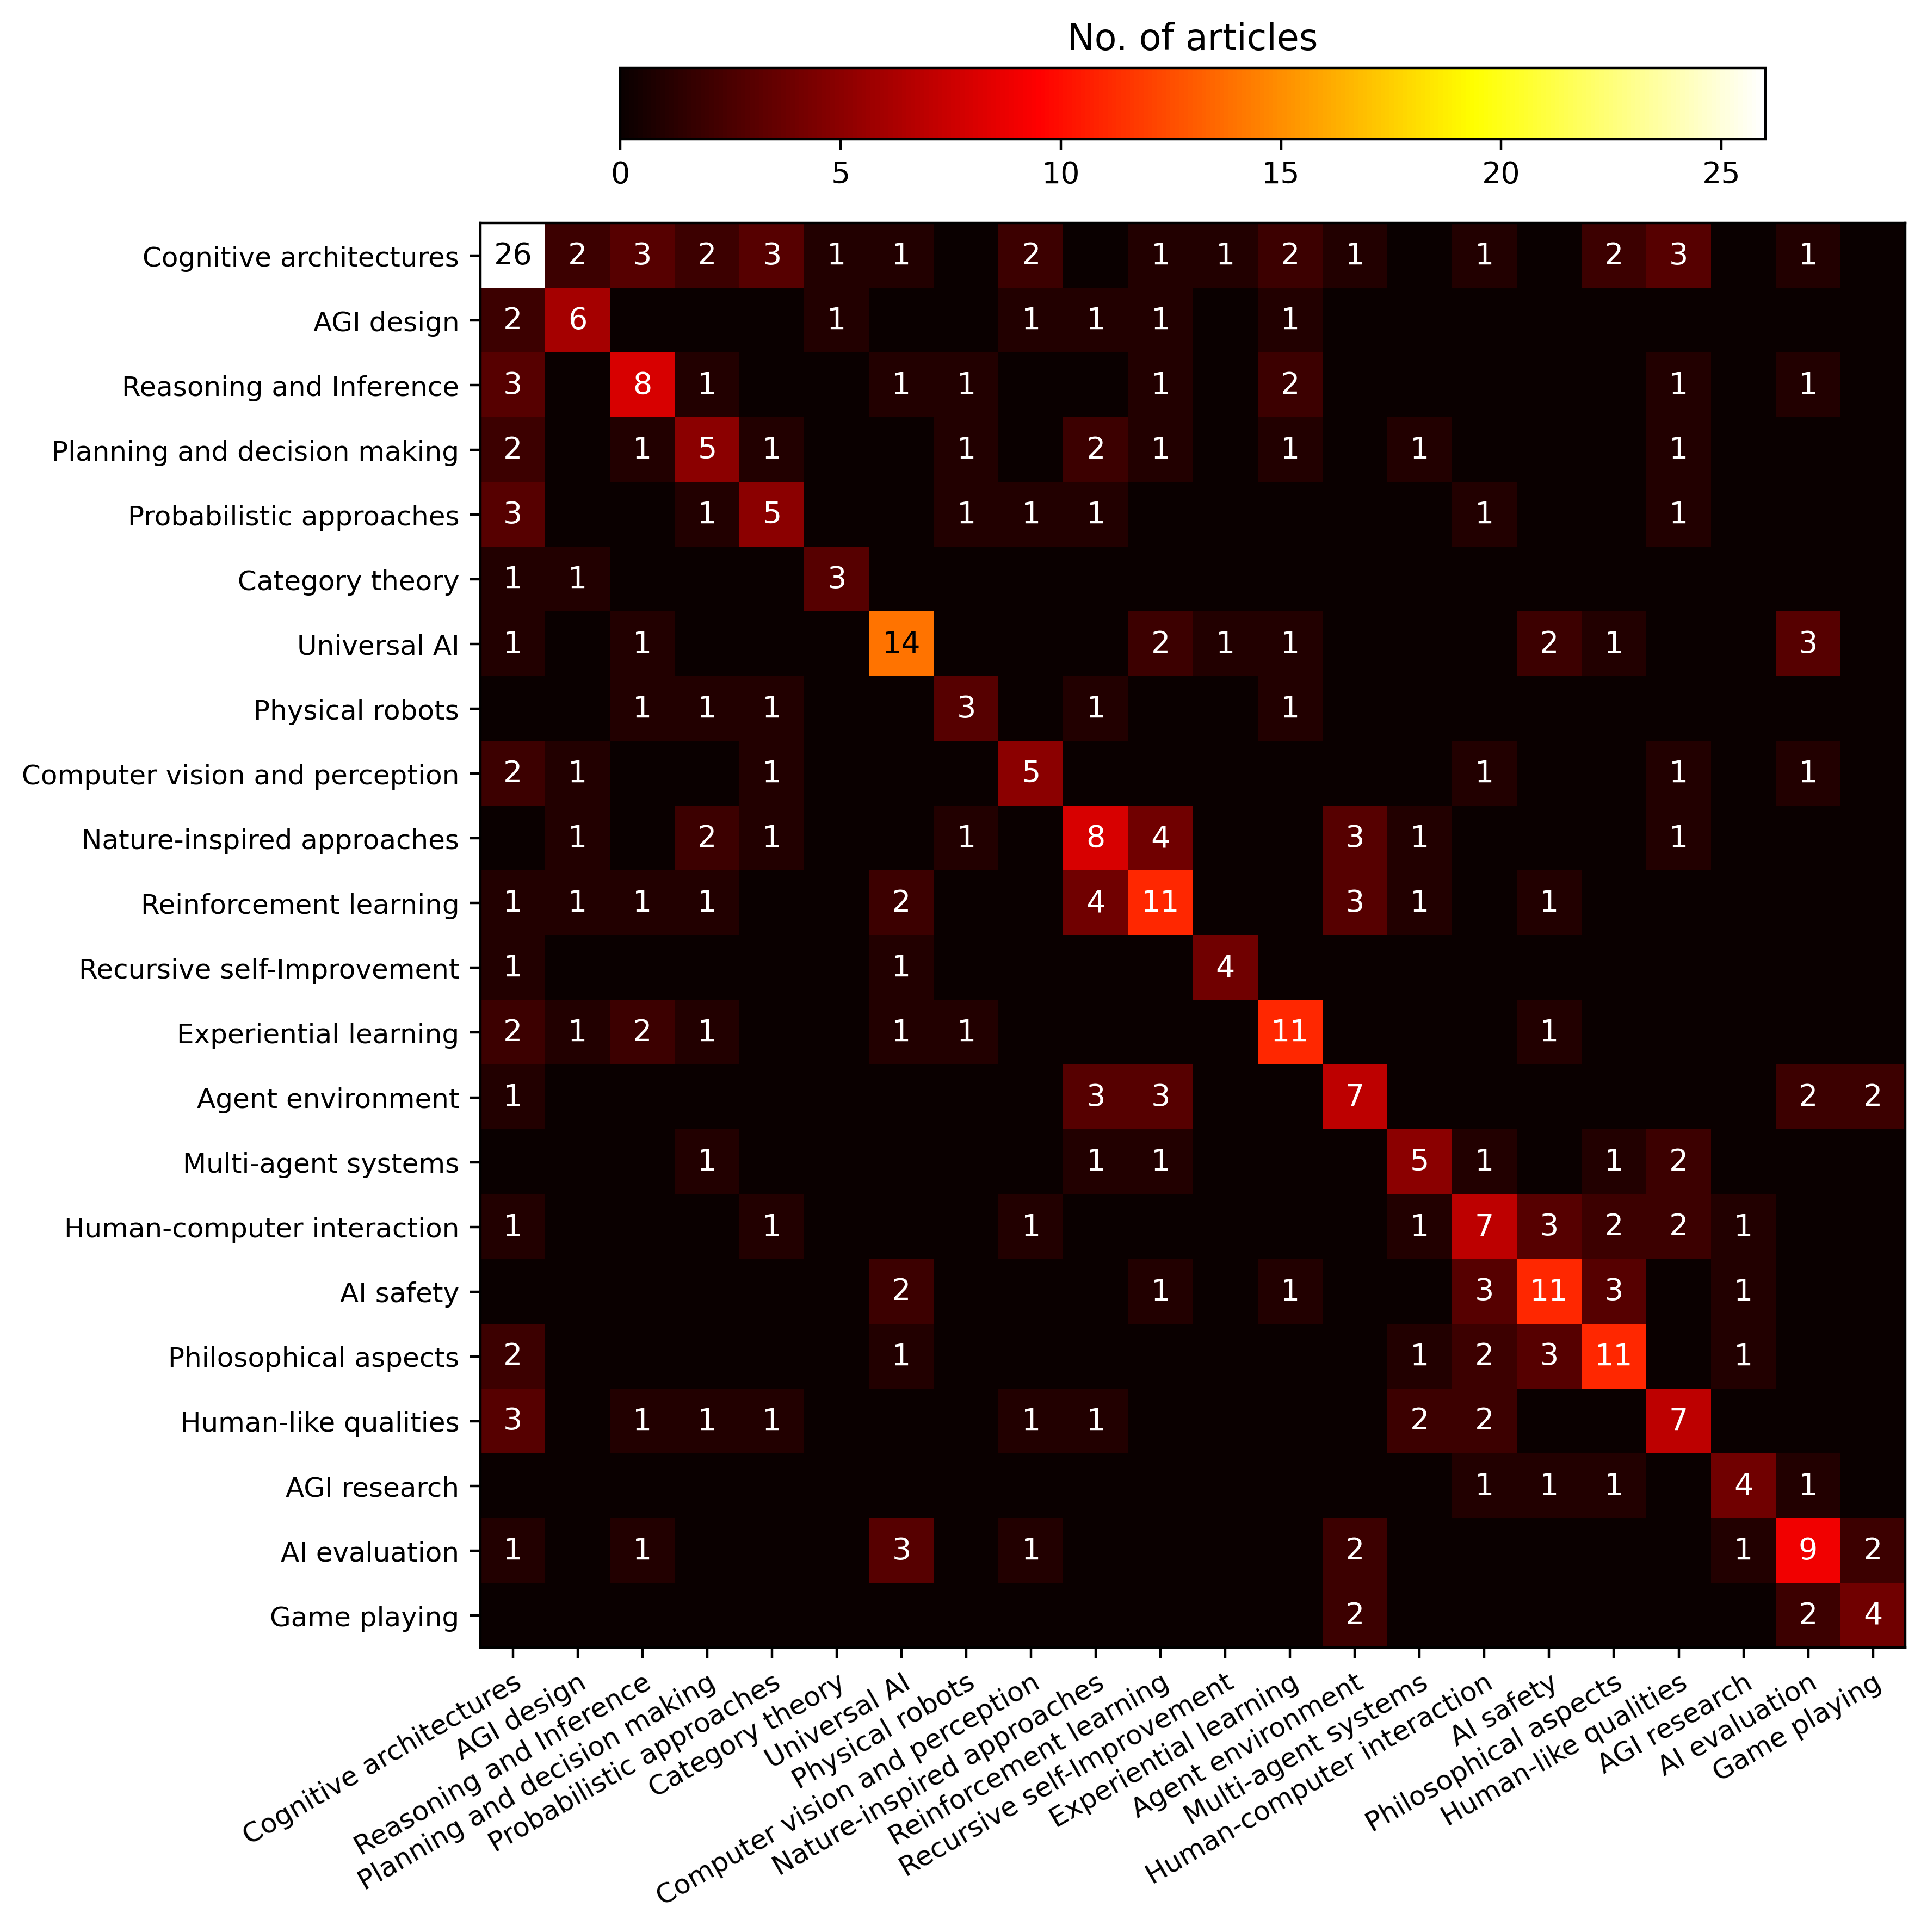
\includegraphics[scale=0.65]{material/data/topic_heatmap_no_zeroes.png}
  \caption{Topic's relations to each other}
  \label{fig:topicheat}
\end{figure}


\section{Types of AGI research}

The bubble graph in Figure \ref{fig:topicbubble} shows us the relation of the
articles' topics and the Wieringa classification. Here we can observe the
specific foci of the field in two different facets.

It can be clearly seen that most of the research in the field is solution
proposals. This means that the research consists predominantly of new approaches
to different problems. This focus on the new ideas combined with the almost
complete lack of evaluation research shows that the field is still very young,
as there is not much practical applications to investigate. It is also possible
that often this kind of evaluation research could be very valuable and therefore
kept private and unpublished, but as the sample articles are mostly from
academia, that should not be the case here. 

There is some validation research, which means investigation of
not-yet-implemented solution proposals. Often solution proposal articles
provided some proof in form of methodological analysis, prototype or
experiments, making them also validation research papers.

Also common were philosophical papers, meaning papers that sketch a new way of
looking at the subject, or that present a conceptual framework to be used in
future research. Especially on the topics of philosophical aspects and AI safety
this was a dominating research type, with multiple ethical frameworks and safety
guidelines presented in the articles. Especially on these topics the lack of
practical applications makes evaluation and validation research difficult, as no
competent AGI exists yet.

To answer the second part of research question RQ1, it can be said that the
research in the AGI field is mostly proposals of new solutions and approaches,
and philosophical papers discussing new conceptual frameworks and views. The
absence of evaluation research shows that the research of existing practical
solutions is nominal, probably due to the fact that the field is challenging and
still focused more on the theoretical side. The lack of opinion papers
also show indicates that the performed research is objective.

The research gap in evaluation research could be target for future research.
Finding examples of AGI solutions used in practice, and investigating their
effectiveness against traditional approaches or more narrow AI solutions would
be an interesting way to survey the state of the field in more detail.
Especially the usage of popular cognitive architectures in real-world situations
could be a good subject for a more focused systematic literature review. 

Topic-wise, physical robots and category theory are the least researched ones.
This is interesting especially when considering the wide usage of robots in
manufacturing and many other industries. There are also recent suggestions that
AGI will never be realized as it cannot experience world as humans can,
attaining tacit knowledge (\cite{fjelland2020why}). Considering this, it would
make sense to invest in a future research that would aim to enable AIs to
experience physical world through robotics. This was also suggested by David
Kremelberg in one of the studied articles (\cite{kremelberg2019embodiment}),
where he argues that embodiment is a necessity for general intelligence.


\pgfplotstableread[col sep=comma, header=true]{material/data/class_topic_bubble.dat}\topicDataTable
\def\forumCoordsFirst{}
\createSymbolicCoords{\forumCoordsFirst}{\topicDataTable}{Category}
\def\classCoordsFirst{}
\createSymbolicCoords{\classCoordsFirst}{\topicDataTable}{Class}
\begin{figure}[H]
  \centering
  \begin{tikzpicture}
    \begin{axis}[
      only marks,
      enlarge x limits=0.06,
      enlarge y limits=0.05,
      width=12cm,
      height=20cm,
      bubbleplot={0.8ex},
      bubbleplot count/.style={font=\footnotesize},
      y tick label style={
          font=\small\linespread{0.8}\selectfont,
          text width=5cm,
          align=right,
          xshift=-0.1cm
        },
      ytick=data,
      symbolic y coords/.expand once={%
          \forumCoordsFirst
        },
      symbolic x coords/.expand once={%
        \classCoordsFirst
        },
      x tick label style={
        font=\tiny\linespread{0.8}\selectfont,
        xshift=0cm,
        },
      scatter
      scatter/@pre marker code/.code={%
      \scope[%
        mark size=#1*(sqrt(\pgfmathfloatvalueof\pgfplotspointmeta)),
        fill=black,%
        color=black,%
      ]
      },
      scatter/@post marker code/.code={%
          \node[/pgfplots/bubbleplot count,color=white]% 
          {\pgfmathprintnumber\pgfplotspointmeta};\endscope
        }]
      \addplot[point meta=explicit] table[x={Class},y={Category},meta={Count},col sep=comma] {\topicDataTable};
    \end{axis}
  \end{tikzpicture}
  \caption{Article distribution between topics and article types}
  \label{fig:topicbubble}
\end{figure}


\section{Research locations}

AI is a issue that has been discussed in mainstream media a lot in the recent
years. Even leaders of many countries have voiced their opinions about the
future prospects of utilizing AI in society. Because of this, although not the
main focus of this thesis, the affiliations of studied articles were also
mapped geographically, and presented in figure \ref{fig:researchmap}. The figure
shows how the research of artificial general intelligence is focused around the
world in different countries. 

With 59 papers published, most of the articles are affiliated with researchers
in European countries. The largest single country in AGI research is USA, with
36 published articles. Suprisingly, Iceland and Netherlands are the runner-ups
with 10 articles each. It can be seen that economic powers like China, Russia
and Japan are still in the 10 largest countries in the field, with 7, 6, and 5
papers respectively. However, their amount of published articles when compared
to that of USA is relatively low. Here it is important to notice that these
numbers do not necessarily reflect the total amount of AI research done, as the
AGI was the focus of the mapping process. Some countries collaborate more than
others, especially Iceland, Switzerland, Netherlands and USA often have articles
involving other nationalities.

It can be observed that there are some authors whose contribution to AGI
research is quite noticeable, based on the number of papers. In Iceland, there's
Kristinn R. Th\'orisson, in China there is Ben Goertzel, in USA there's Pei Wang
and Patrick Hammer, and also many others. Naturally their work is often relating
to same subject, in this case, cumulative learning, OpenCog, and NARS,
respectively.

The complete list of countries can be found in
appendix \ref*{tab:countrypapers}. There was also one paper with no affiliated
country, released by Microsoft's research group.

\begin{sidewaysfigure}[hbtp]
  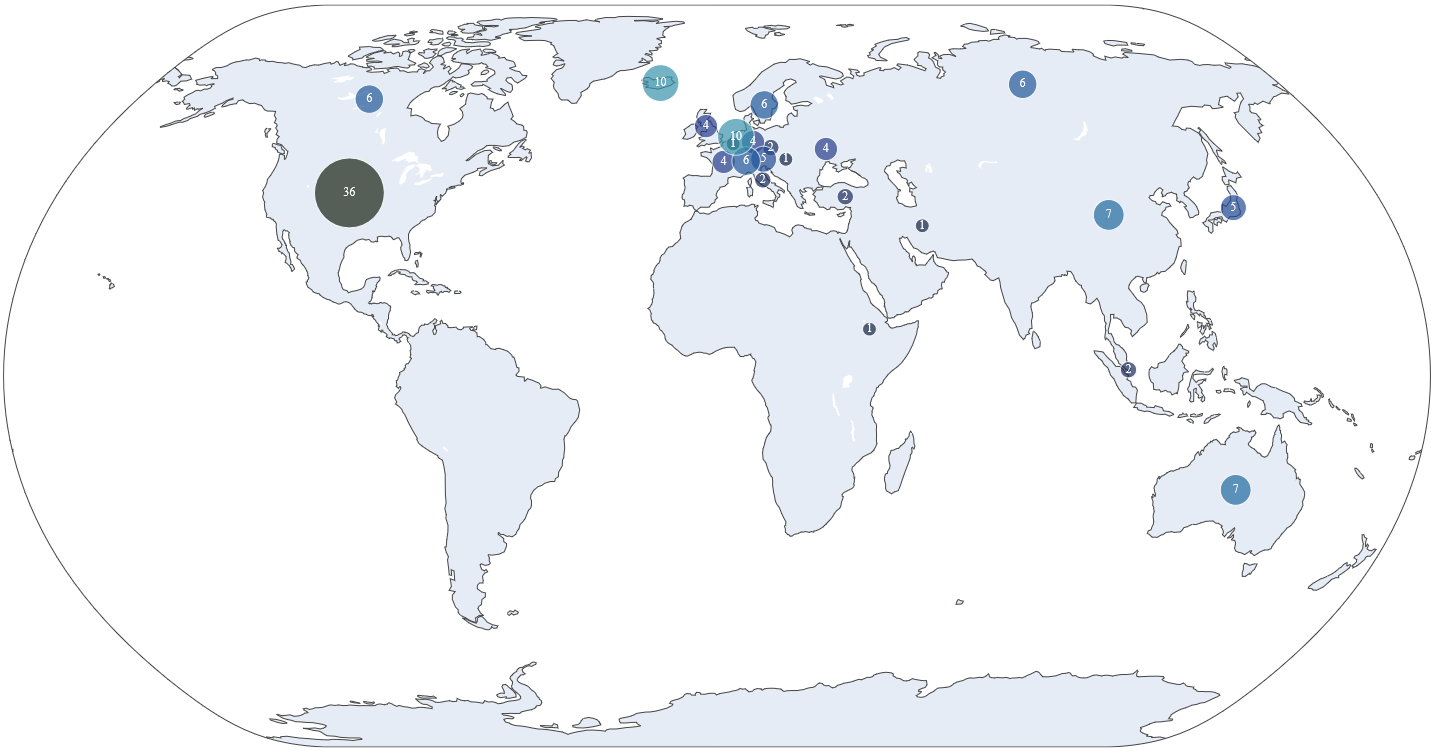
\includegraphics[scale=0.60]{material/data/research_map_delta_count.png}
  \caption{Article affiliation map}
  \label{fig:researchmap}
\end{sidewaysfigure}

\chapter{Conclusion}
\label{chap:conclusion}

In this thesis, a systematic literature mapping study was conducted on the field
of artificial general intelligence. The goal was to create a general overview of
the complex AGI research field and to uncover its current state. 

92 peer-reviewed articles from scientific journals and conference proceedings
were inspected. With three journals and two conferences examined, it was found
out that majority of AGI research is published as the proceedings of the
International Conference on Artificial General Intelligence and in the Journal
of Artificial General Intelligence, with a shares of 85.87\% and 6.52\%,
respectively. The AGI research is focused on these two venues, as the more
general forums constitute only 7.61\% of the publications.

During the inspected years 2015-2019, an average of 18,4 articles were published
yearly, with some fluctuation in different years. While popular topics remain
relatively well represented each year, there are topics like probabilistic
approaches, that haven't been seen in the articles since 2016.

Through the mapping process, 22 distinct topical categories were found. Major
themes in the research are development of AGI systems, different types of
learning, interaction of agents, and philosophical questions about AI. Topics
that stood out the most were cognitive architectures, universal AI,
reinforcement learning, experiental learning, and AI safety and ethics.
Cognitive architecture frameworks and implementations like OpenCog and NARS are
heavily researched, with 26 articles relating to them directly. Universal AI,
which comprises subjects like universal induction and AIXI, is the second most
researched topic with 14 relating papers. It is also interesting to see that as
the dangers of AI and "intelligence explosion" are subjects often discussed in
the media, AI safety is also one of the most researched topics in the field of
AGI.

When viewed through scientific paper classification by Wieringa et al.
(\cite{wieringa2006}), the current AGI research is mostly solution proposals,
presenting new ideas and approaches to problems. The lack of evaluation research
shows that there is not yet much practical applications to evaluate. The
ultimate goal of AGI is not yet realized and the complete absence of industry
applications is a worrying sign of slow progress.

Philosophical papers presenting conceptual frameworks and new views are also
common in the field. AI safety, meaning how to control and contain
superintelligent agent, and ethical questions about values and the relationship
between the man and the machine are clearly things that require discussion.

When placing the AGI research on the geographic map, it is apparent that most of
the explorations in the field is performed by researchers in Europe and United
States of America. In Europe, nations standing out are Iceland and Netherlands,
both publishing more articles on the subject than Russia, China and Japan. This
may not however reflect the amount of other AI research.

When future AGI research is concerned, the research gaps observed through the
mapping would suggest that there is a need for more research on practical
applications of AGI, if there are any. This would truly show the current state
of progress, and could help the growth of interest in the area. It is also seen
that there are only few studies combining robotics with AGI, and as there are
suggestions that having a physical body is required for human-like learning, it
would make sense to further investigate this subject as well.

In this mapping study, it was observed that while AGI research is definitely not
very popular subfield of AI at the moment, there is steady amount of articles
being published on the topics regularly in its main publication forums, with
wide variety of different issues.It is however obvious that even though there
have been major breakthroughs in AI in recent years, the ultimate goal of
general intelligence is not yet close to realization.



\printbibliography

\appendix

\section{Accepted papers}
\label{tab:acceptedpapers}
\begin{longtable}{|>{\scriptsize}l|>{\scriptsize}p{3cm}|>{\scriptsize}p{5.5cm}|>{\scriptsize}p{2.4cm}|>{\scriptsize}p{2.4cm}|} 
 \hline
 \textbf{Year} & \textbf{Authors} & \textbf{Title} & \textbf{Class} & \textbf{Categories} \\\hline\hline
 \csvreader[separator=semicolon,late after line=\\\hline]%
 {material/data/accepted_papers.csv}{year=\yeari,authors=\authorsi,title=\titlei,class=\classi,categories=\categoriesi}%
 {\yeari & \authorsi & \titlei & \classi & \categoriesi}%
\end{longtable}


\section{Article count per country}
\label{tab:countrypapers}

\begin{table}[H]
\footnotesize  
\begin{tabular}{|l|c|}
 \hline
 \textbf{Country} & \textbf{Article count}\\\hline\hline
 \csvreader[late after line=\\\hline]%
 {material/data/country_data_desc.csv}{country=\country,count=\count}%
 {\country & \count}%
\end{tabular}
\end{table}
  

\end{document}